\subsection{Rate-limited, repetition 1}
\begin{figure}[H]\centering
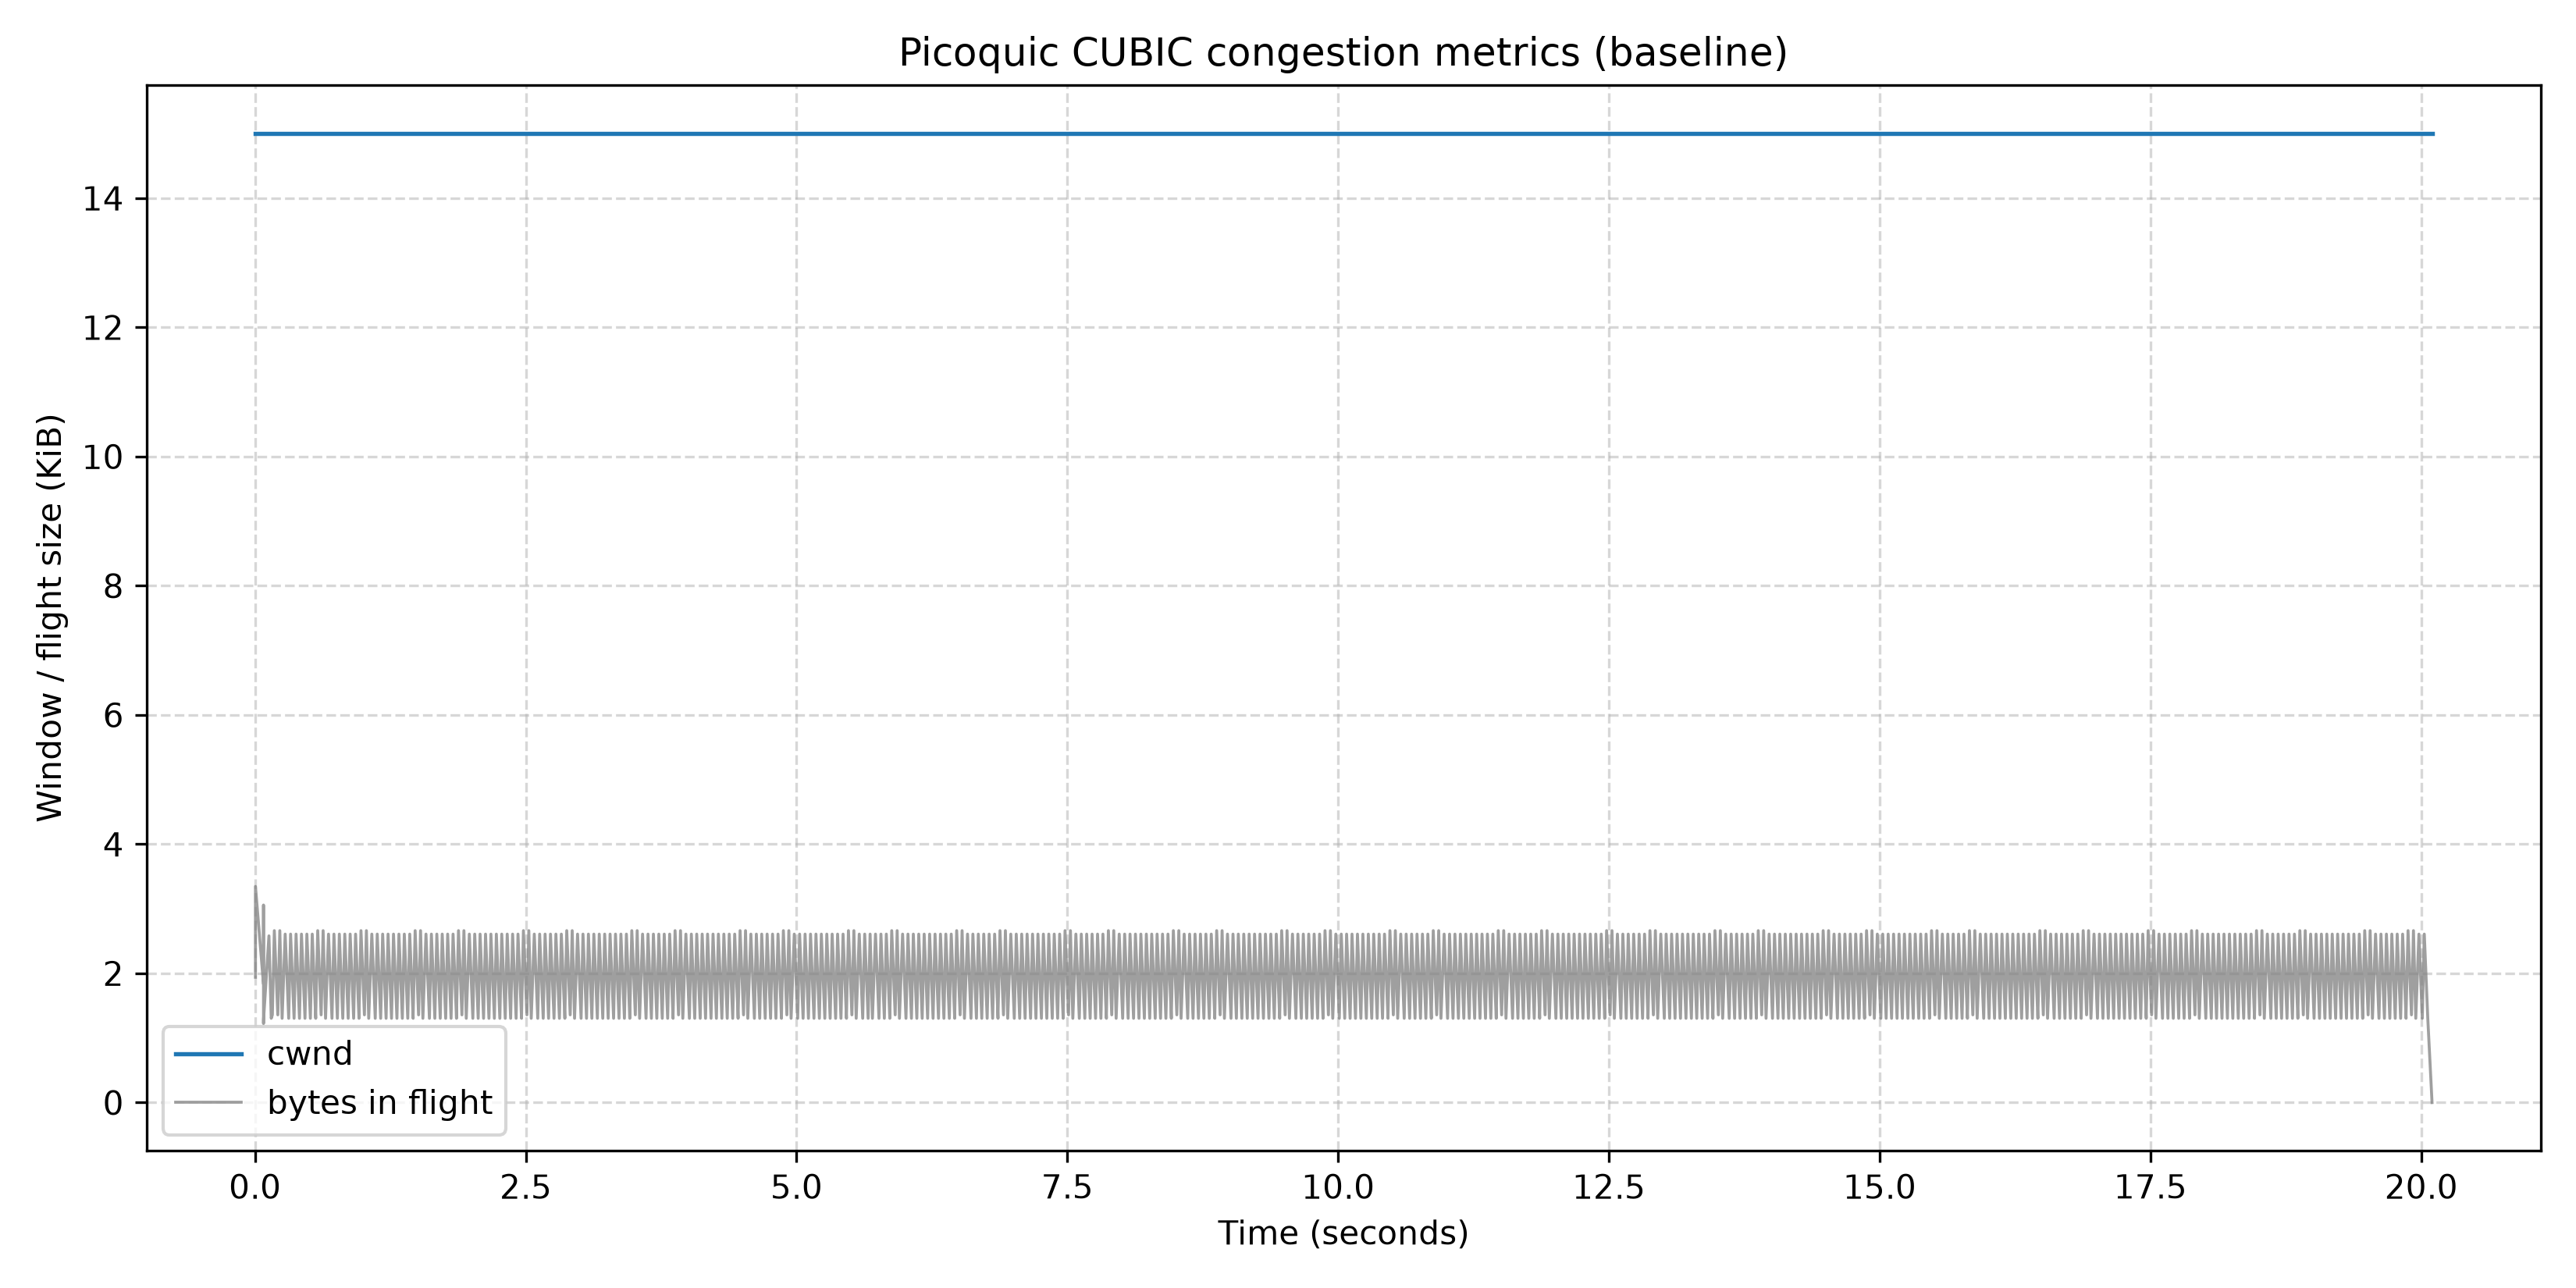
\includegraphics[width=0.92\textwidth]{plots/rate-limited-baseline-1.png}
\caption{Baseline: final cwnd 15.00 KiB; time-weighted mean 15.00 KiB; throughput 0.189 Mbit/s.}\end{figure}
\begin{figure}[H]\centering
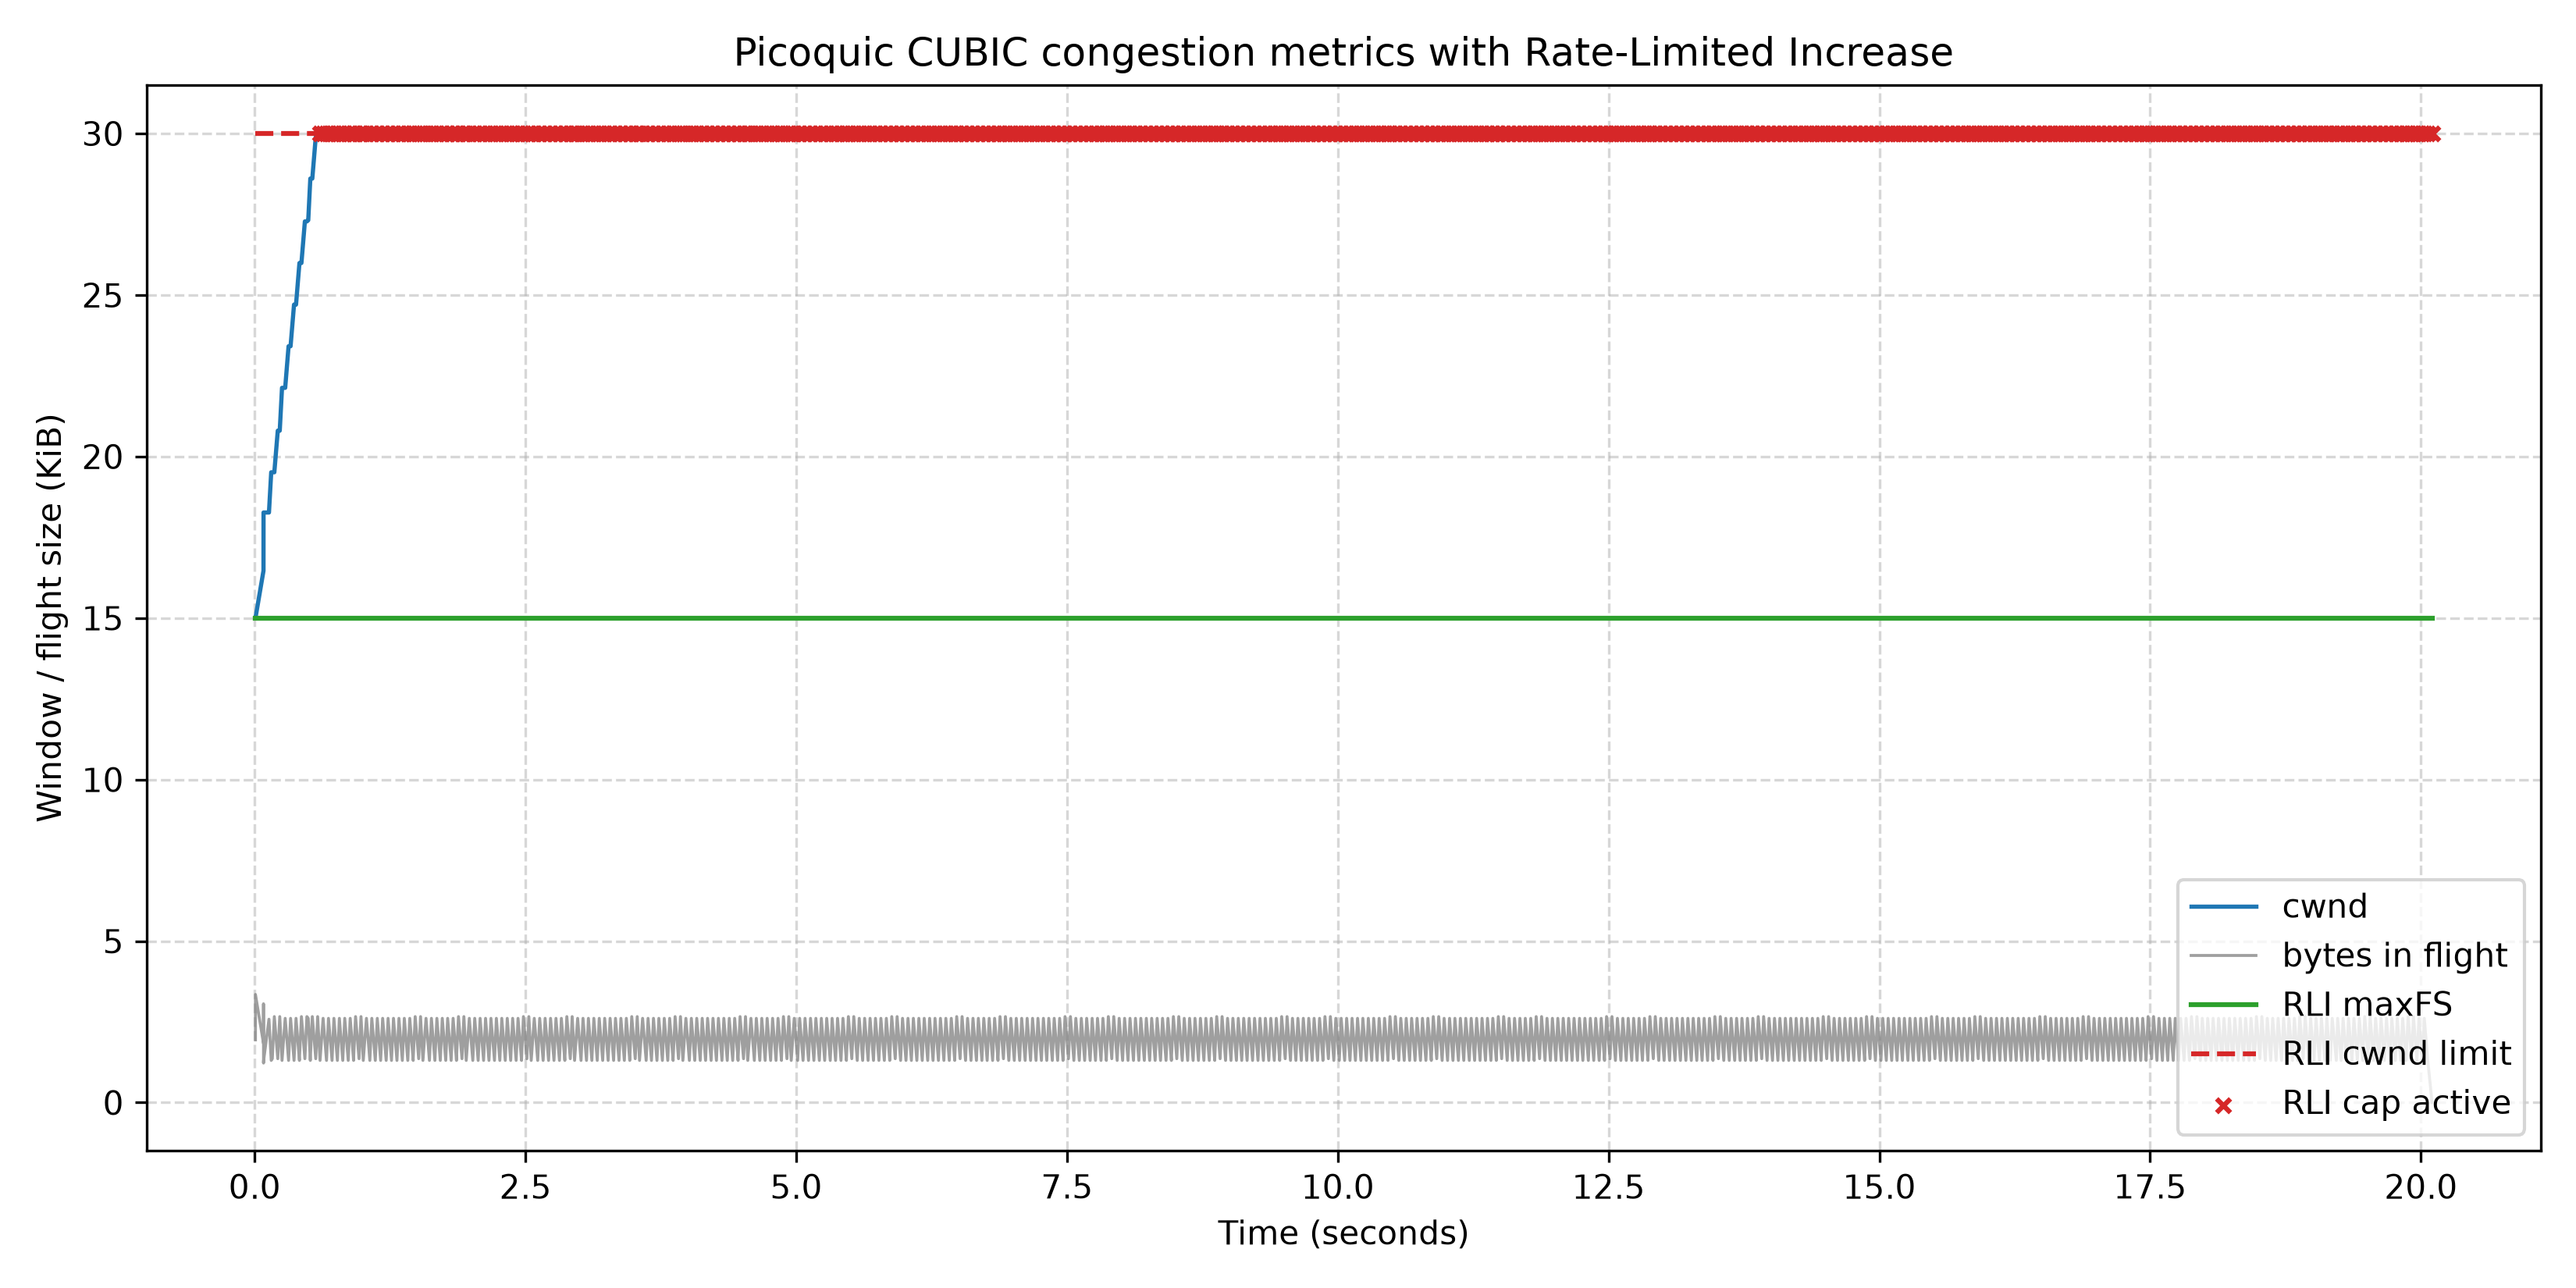
\includegraphics[width=0.92\textwidth]{plots/rate-limited-rli-1.png}
\caption{Rli: final cwnd 30.00 KiB; time-weighted mean 29.78 KiB; throughput 0.189 Mbit/s.}\end{figure}
These matched traces isolate rate-limited window growth. RLI permits bounded ACK-driven growth; application supply still controls throughput.
\clearpage\subsection{Rate-limited, repetition 2}
\begin{figure}[H]\centering
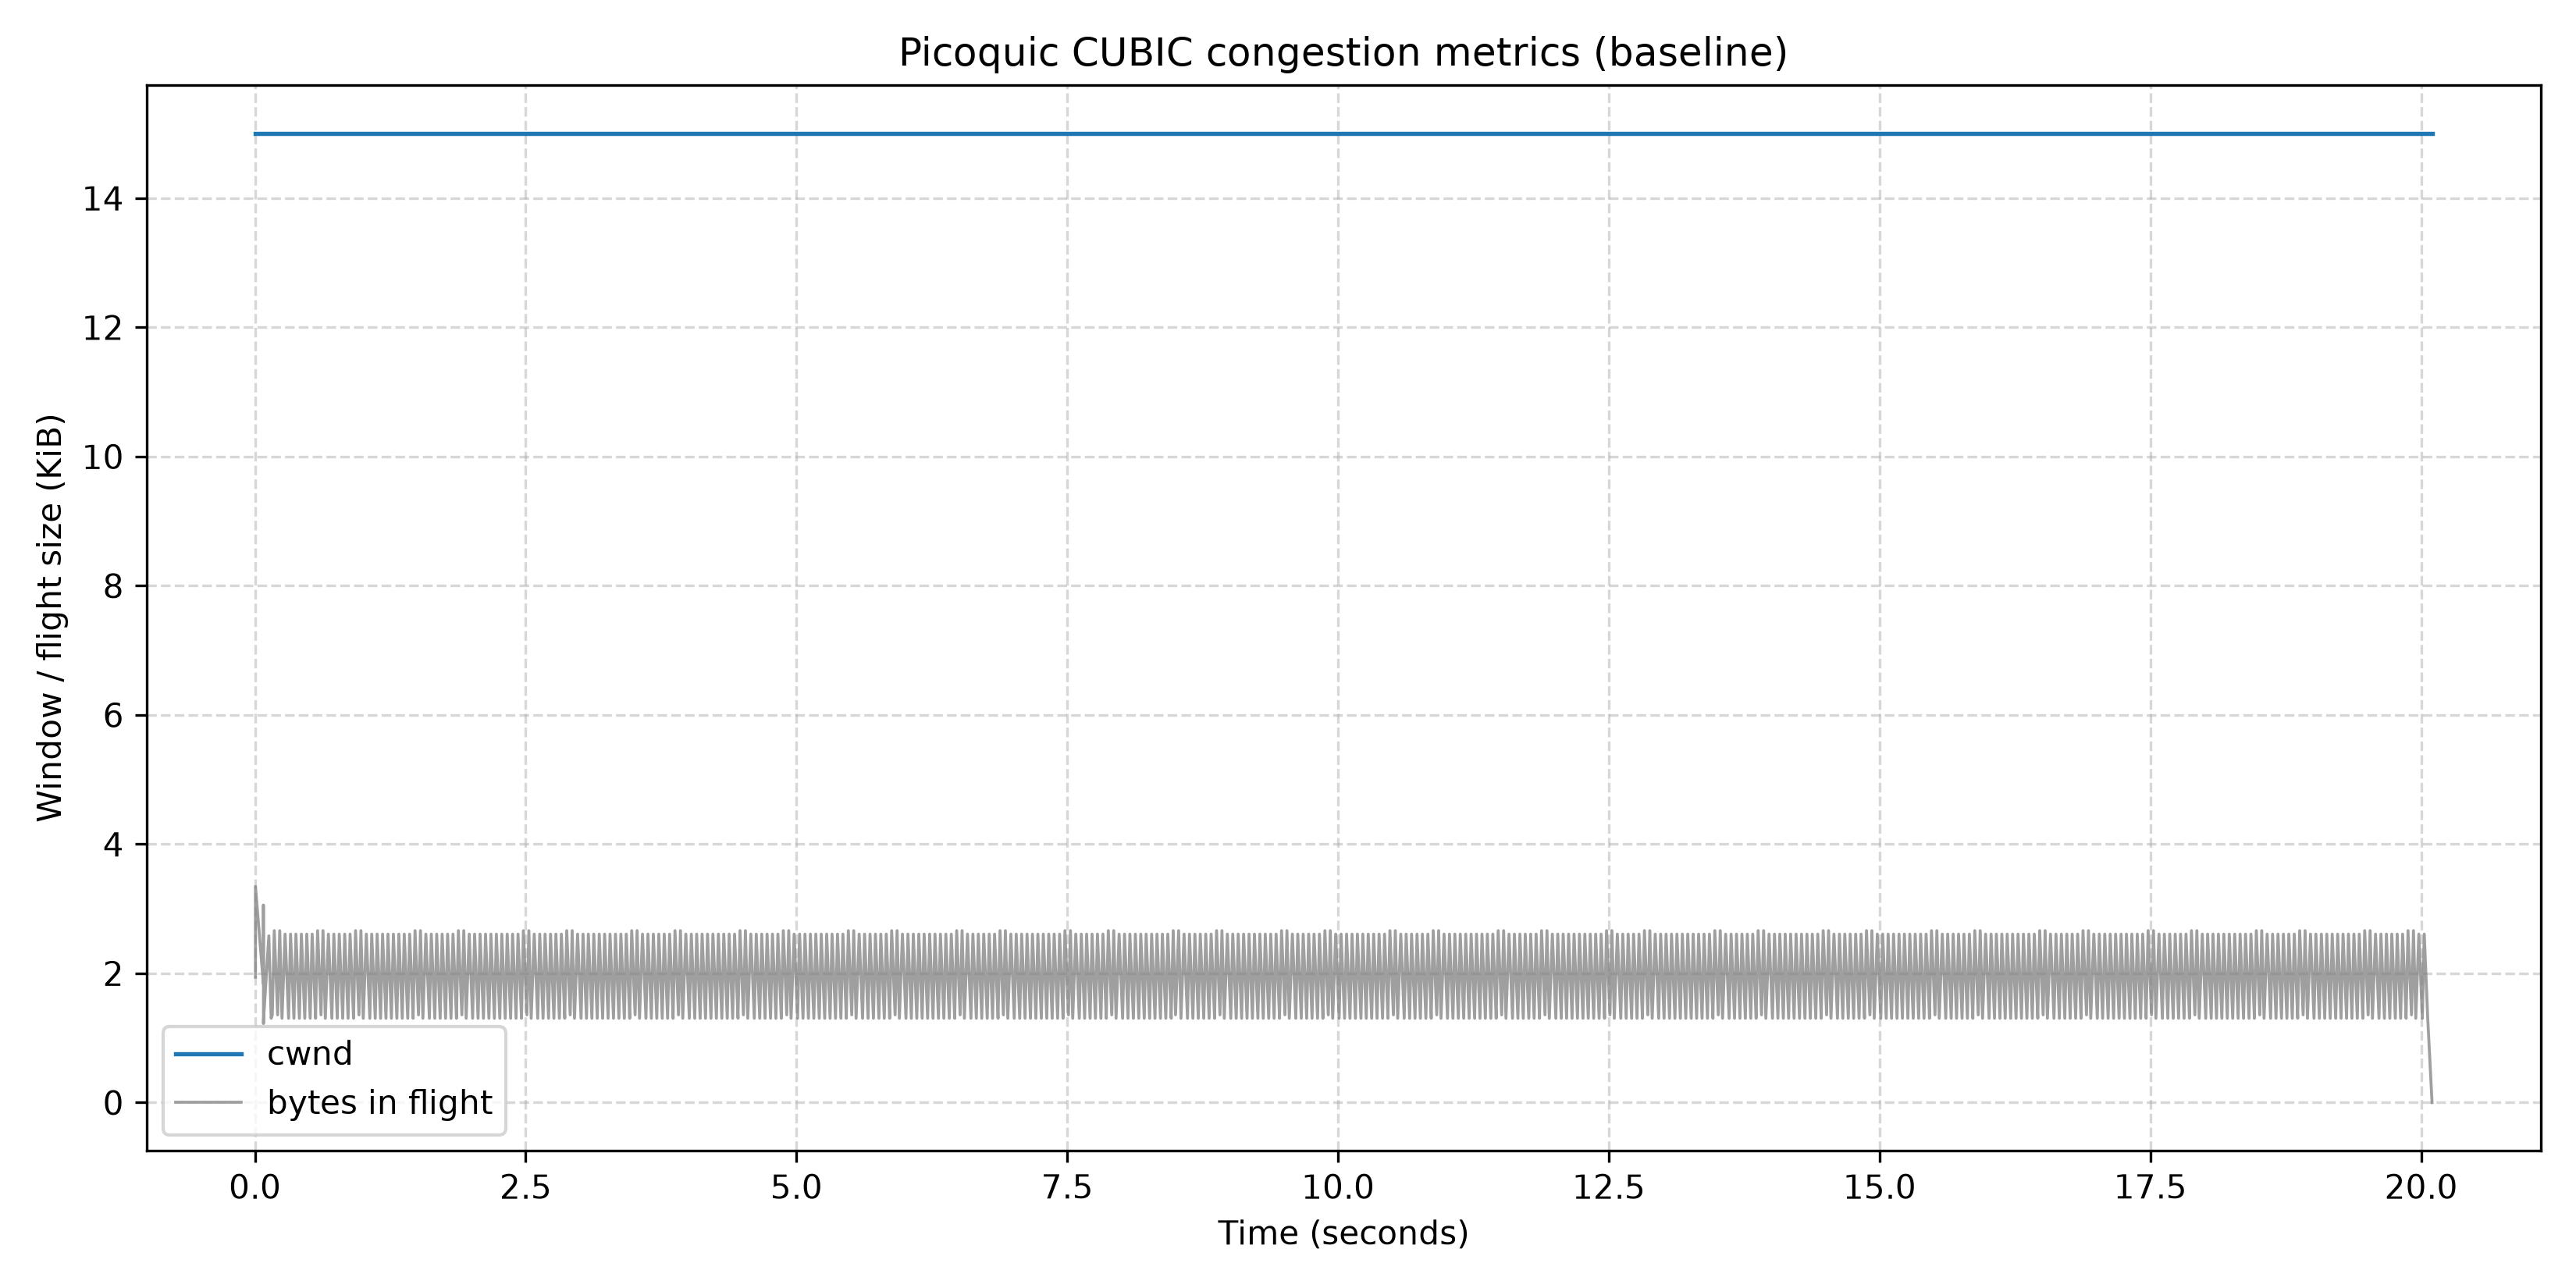
\includegraphics[width=0.92\textwidth]{plots/rate-limited-baseline-2.png}
\caption{Baseline: final cwnd 15.00 KiB; time-weighted mean 15.00 KiB; throughput 0.189 Mbit/s.}\end{figure}
\begin{figure}[H]\centering
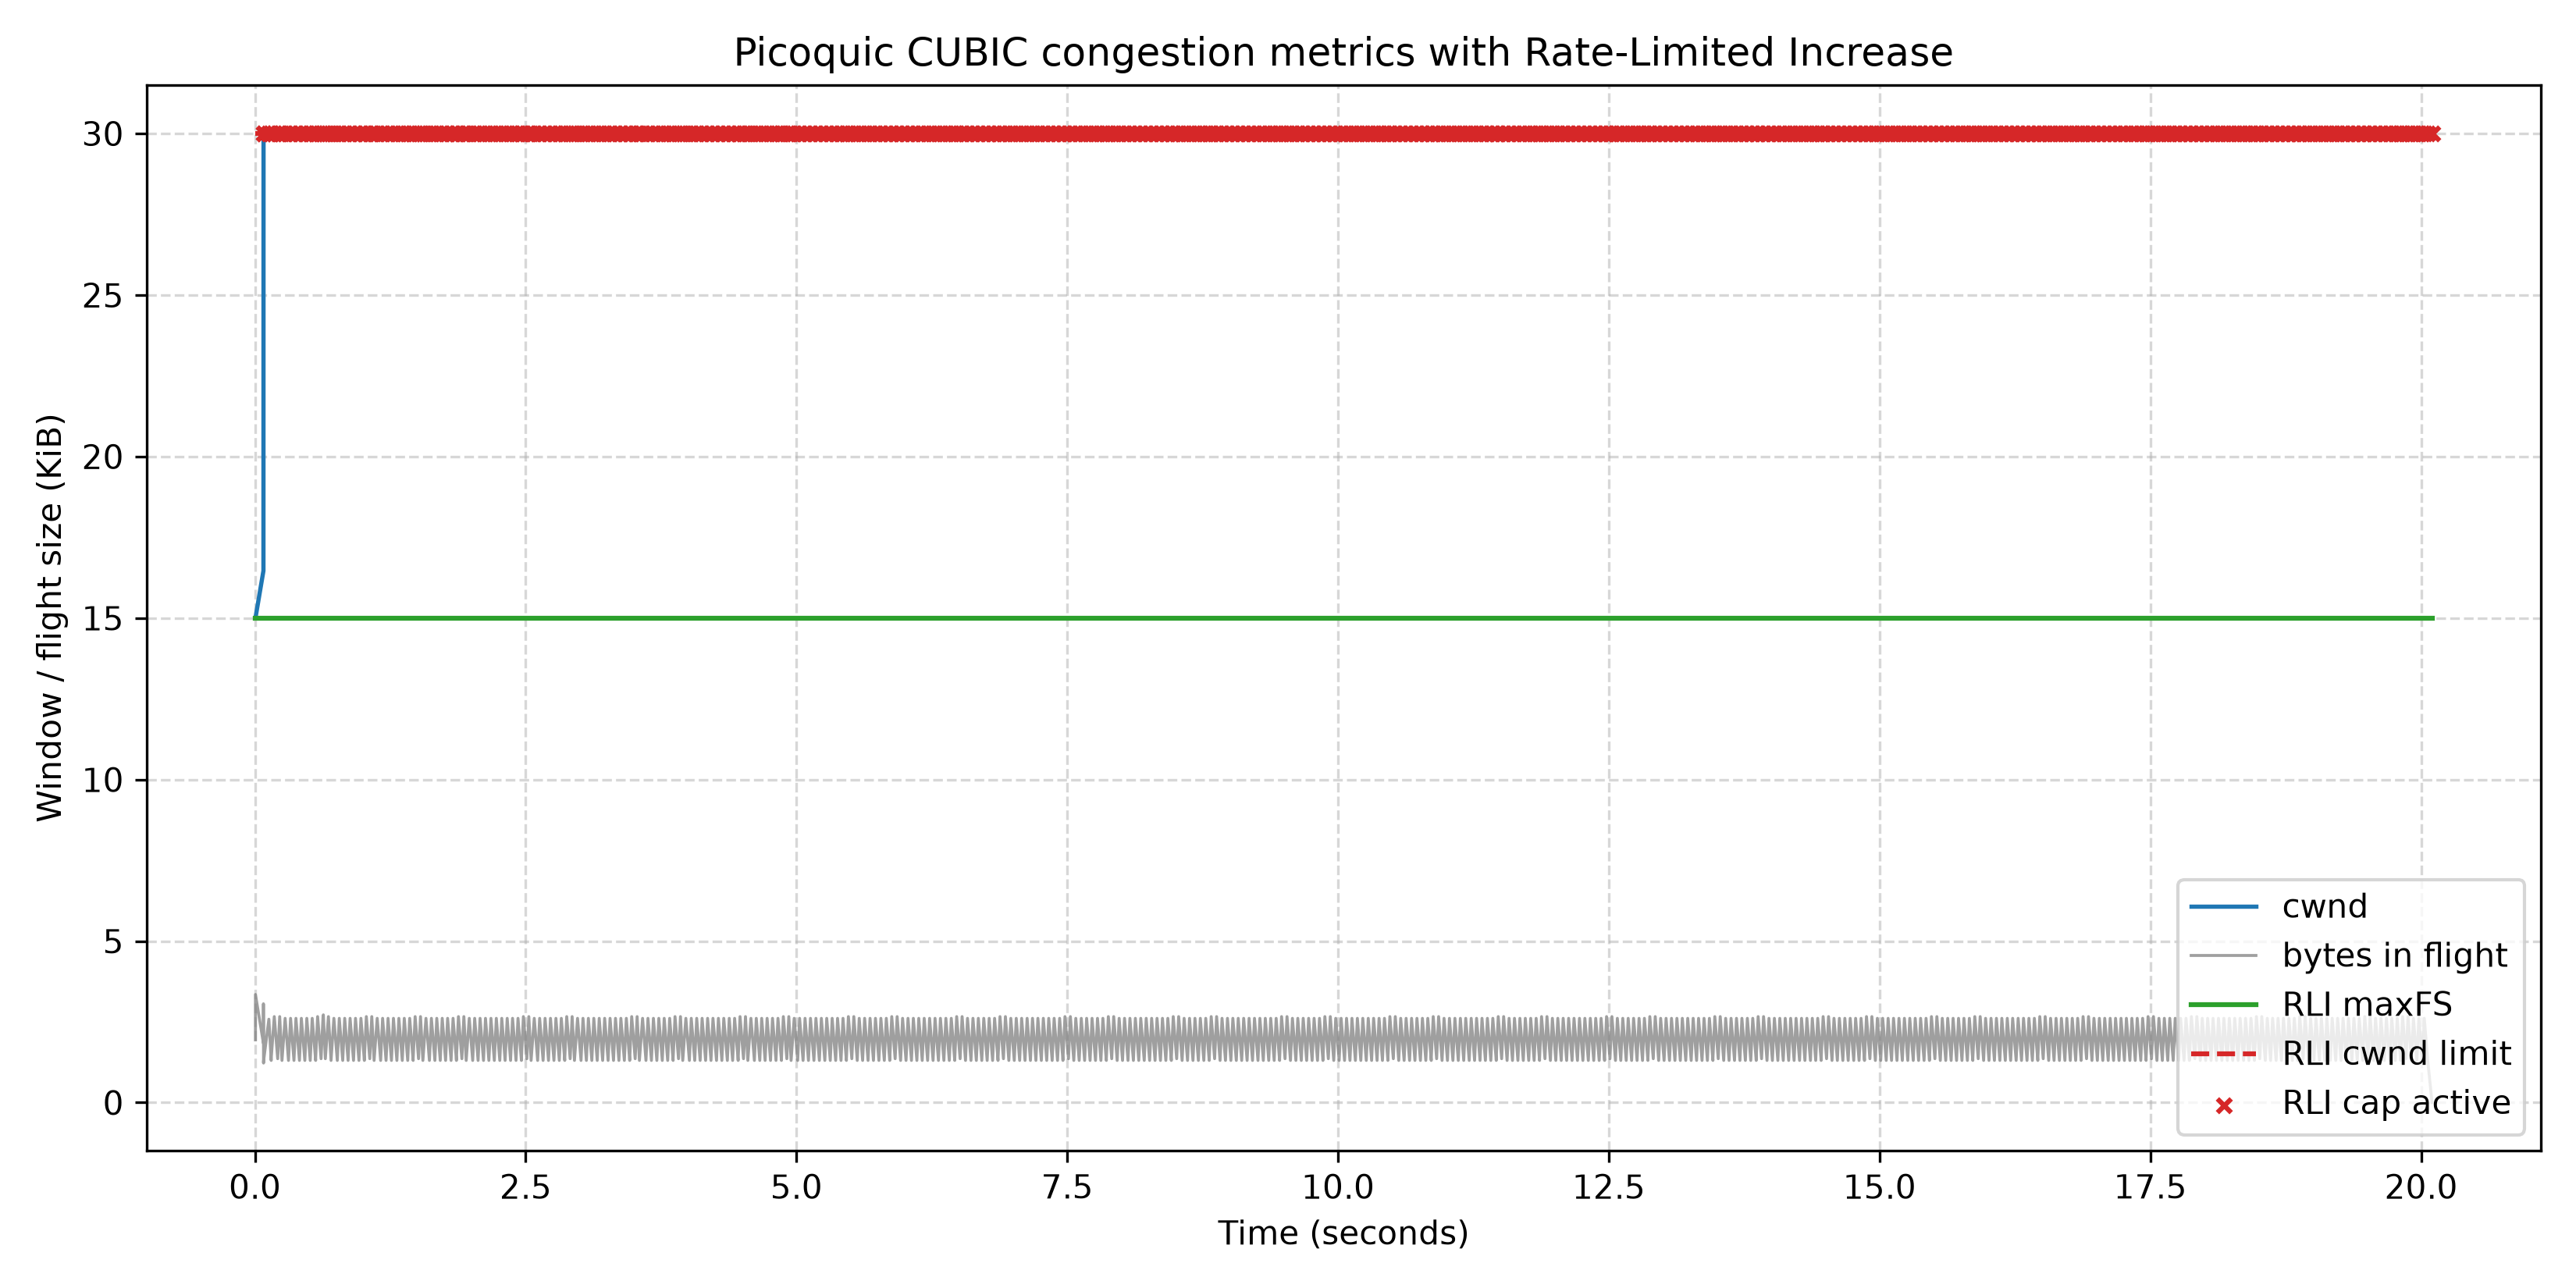
\includegraphics[width=0.92\textwidth]{plots/rate-limited-rli-2.png}
\caption{Rli: final cwnd 30.00 KiB; time-weighted mean 29.94 KiB; throughput 0.189 Mbit/s.}\end{figure}
These matched traces isolate rate-limited window growth. RLI permits bounded ACK-driven growth; application supply still controls throughput.
\clearpage\subsection{Rate-limited, repetition 3}
\begin{figure}[H]\centering
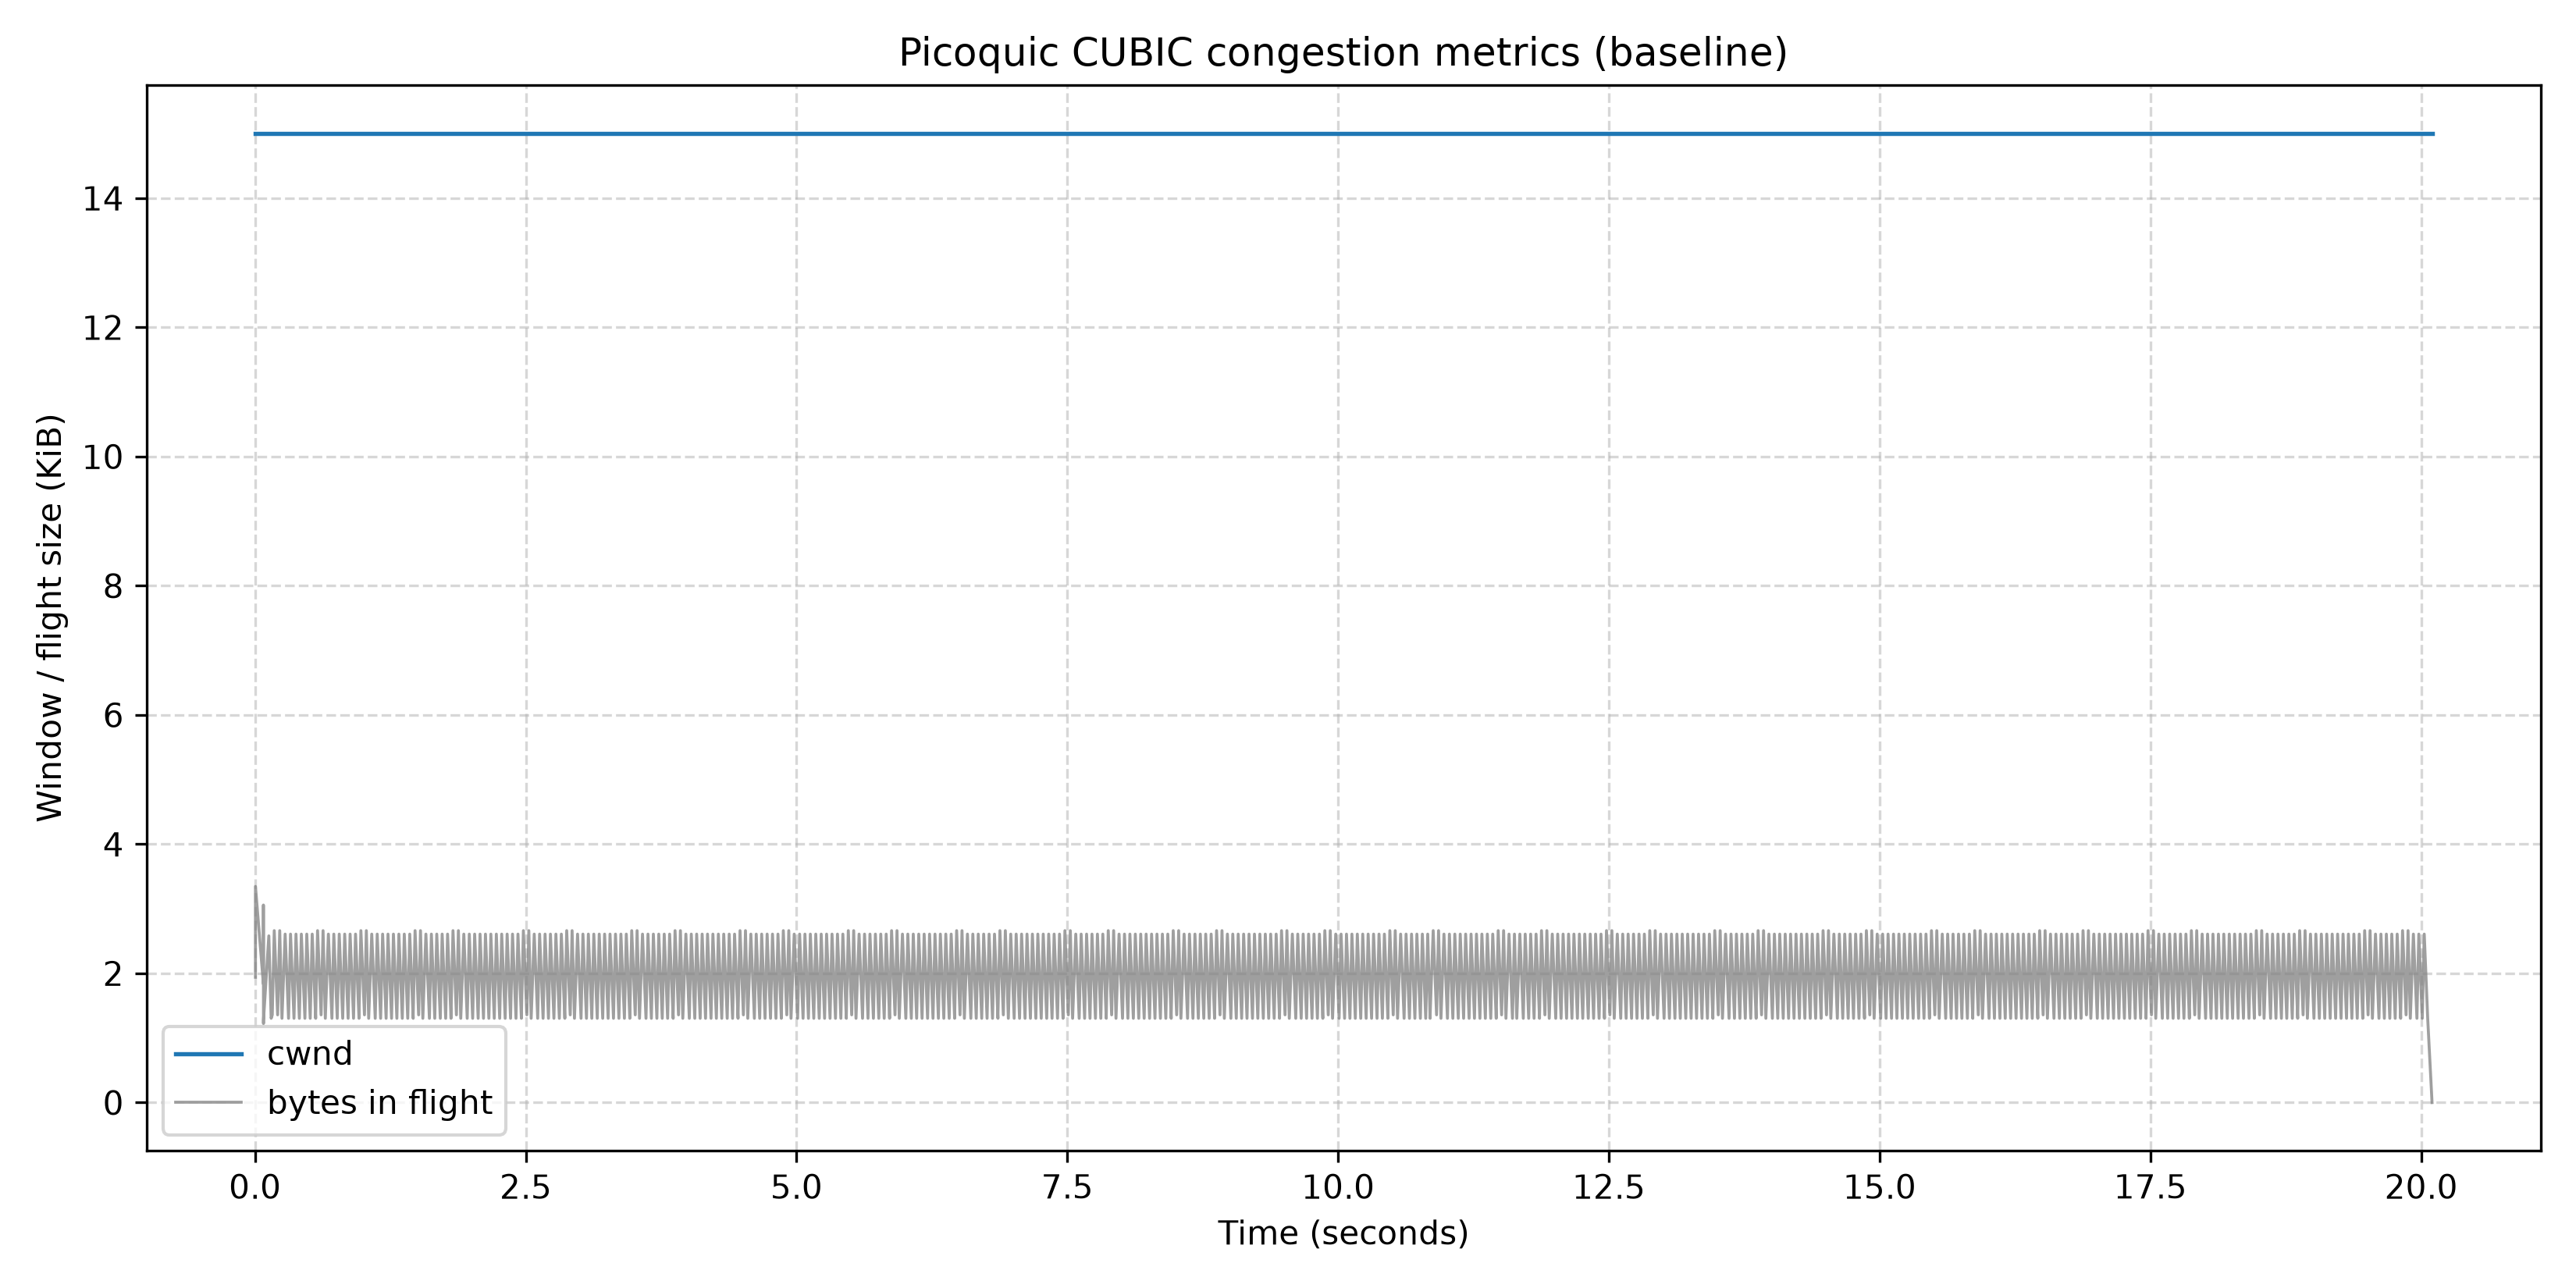
\includegraphics[width=0.92\textwidth]{plots/rate-limited-baseline-3.png}
\caption{Baseline: final cwnd 15.00 KiB; time-weighted mean 15.00 KiB; throughput 0.189 Mbit/s.}\end{figure}
\begin{figure}[H]\centering
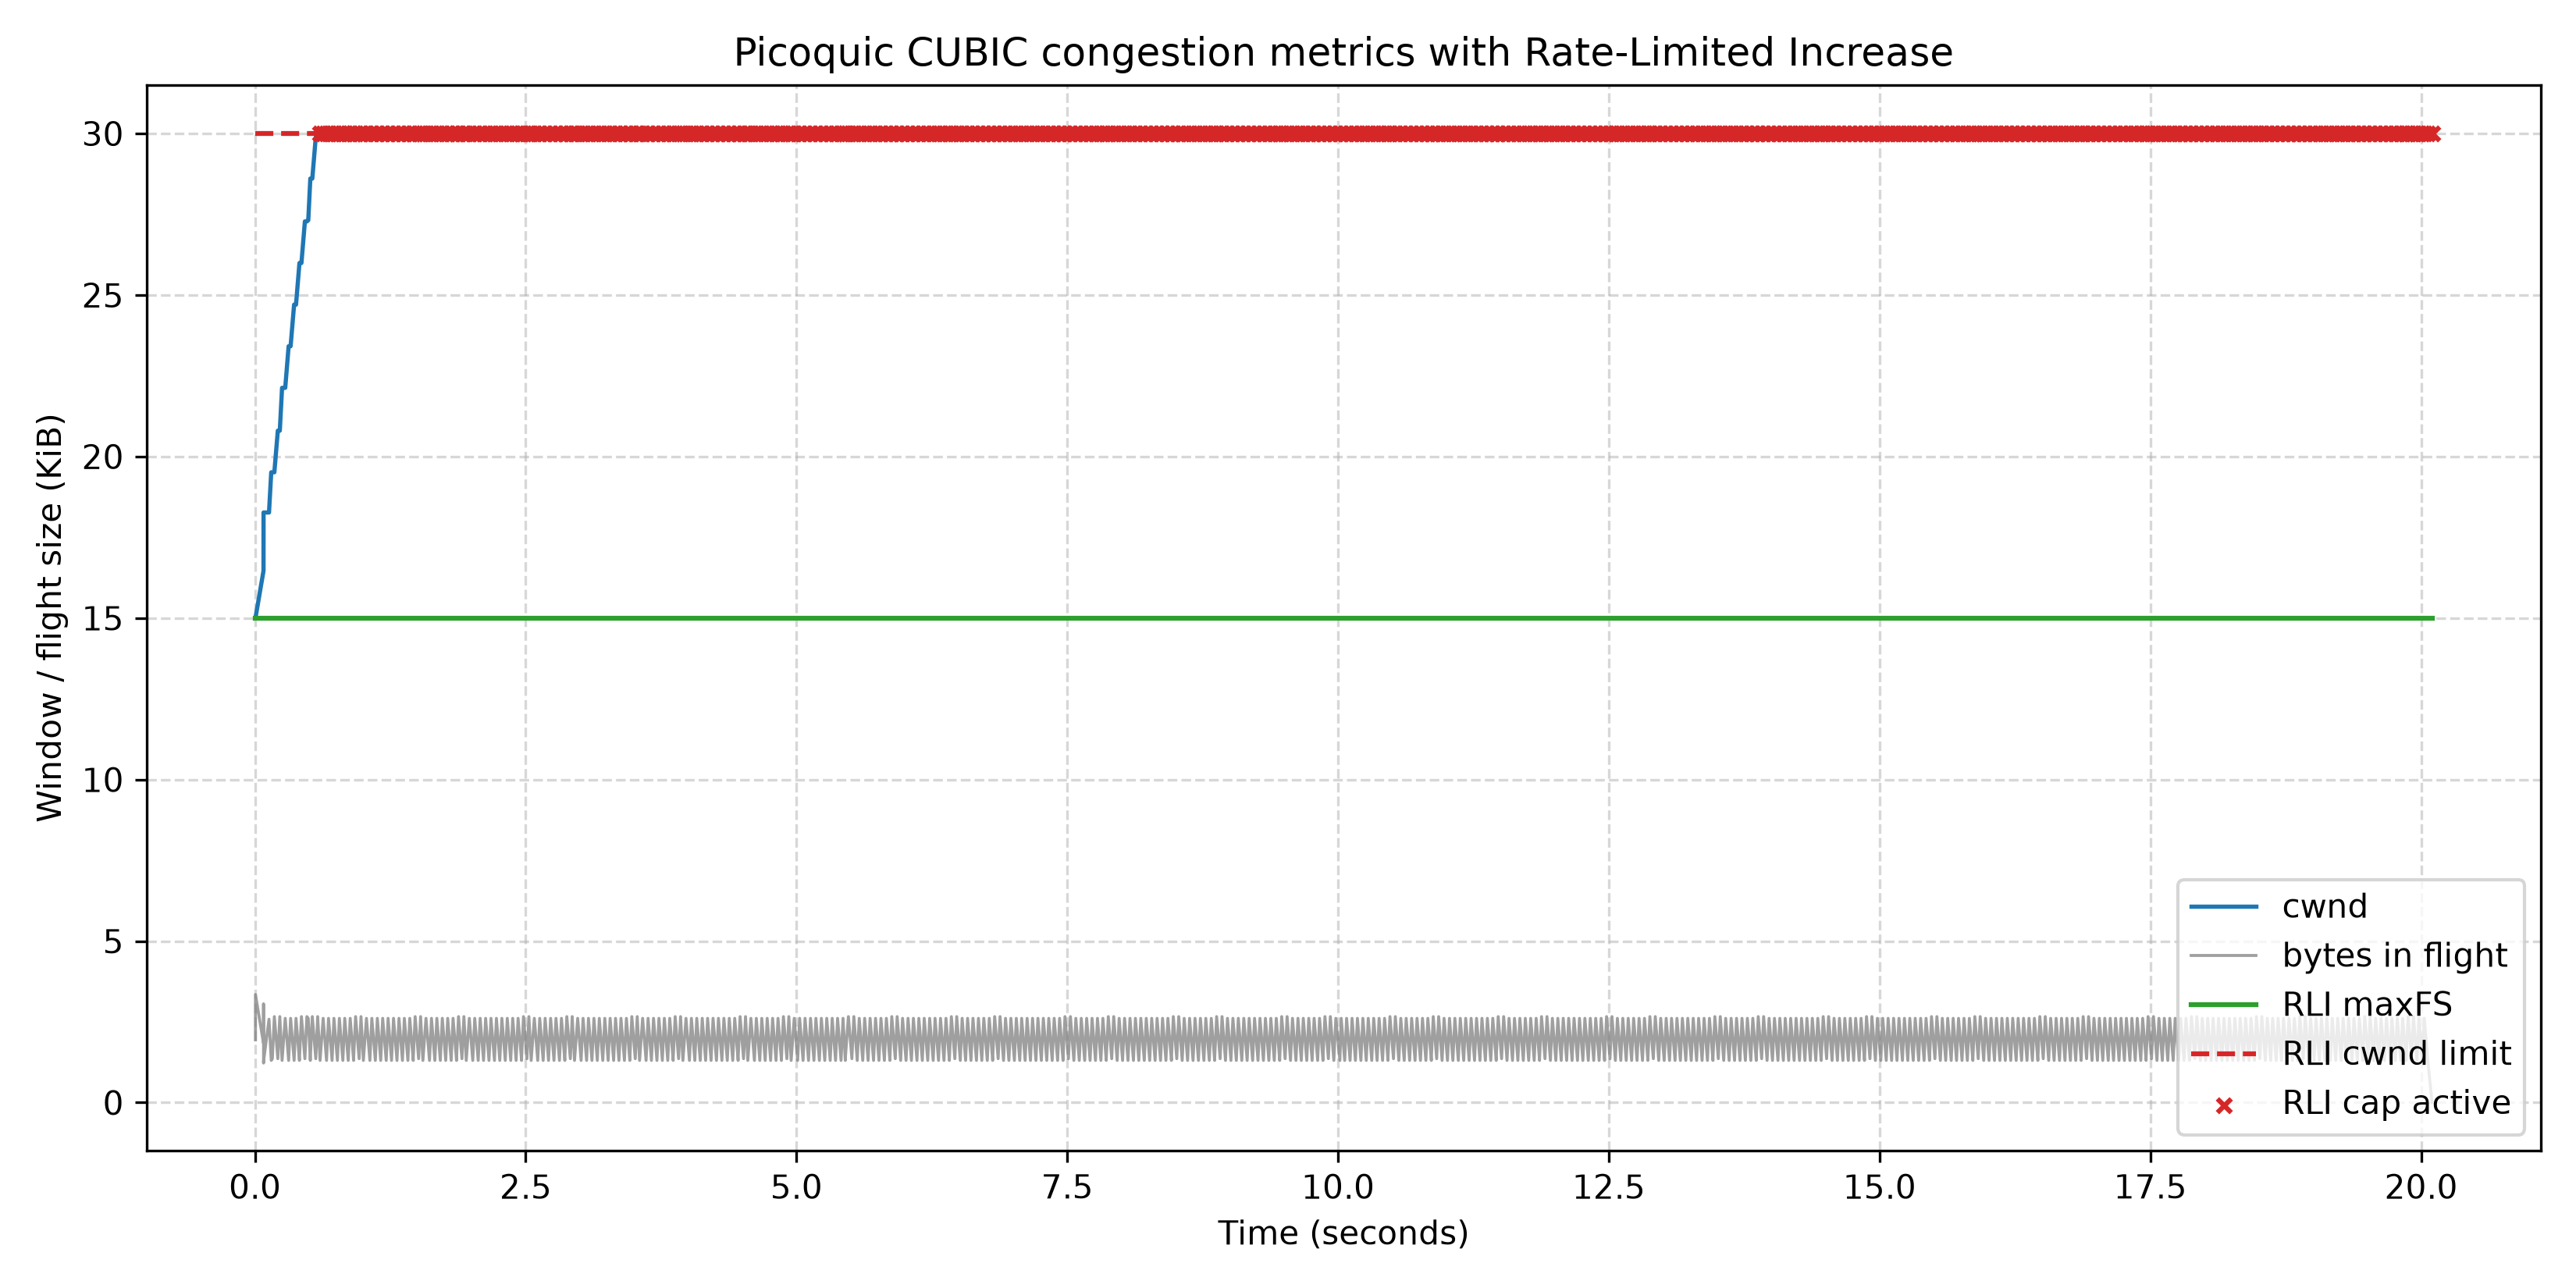
\includegraphics[width=0.92\textwidth]{plots/rate-limited-rli-3.png}
\caption{Rli: final cwnd 30.00 KiB; time-weighted mean 29.78 KiB; throughput 0.189 Mbit/s.}\end{figure}
These matched traces isolate rate-limited window growth. RLI permits bounded ACK-driven growth; application supply still controls throughput.
\clearpage\subsection{Bulk control, repetition 1}
\begin{figure}[H]\centering
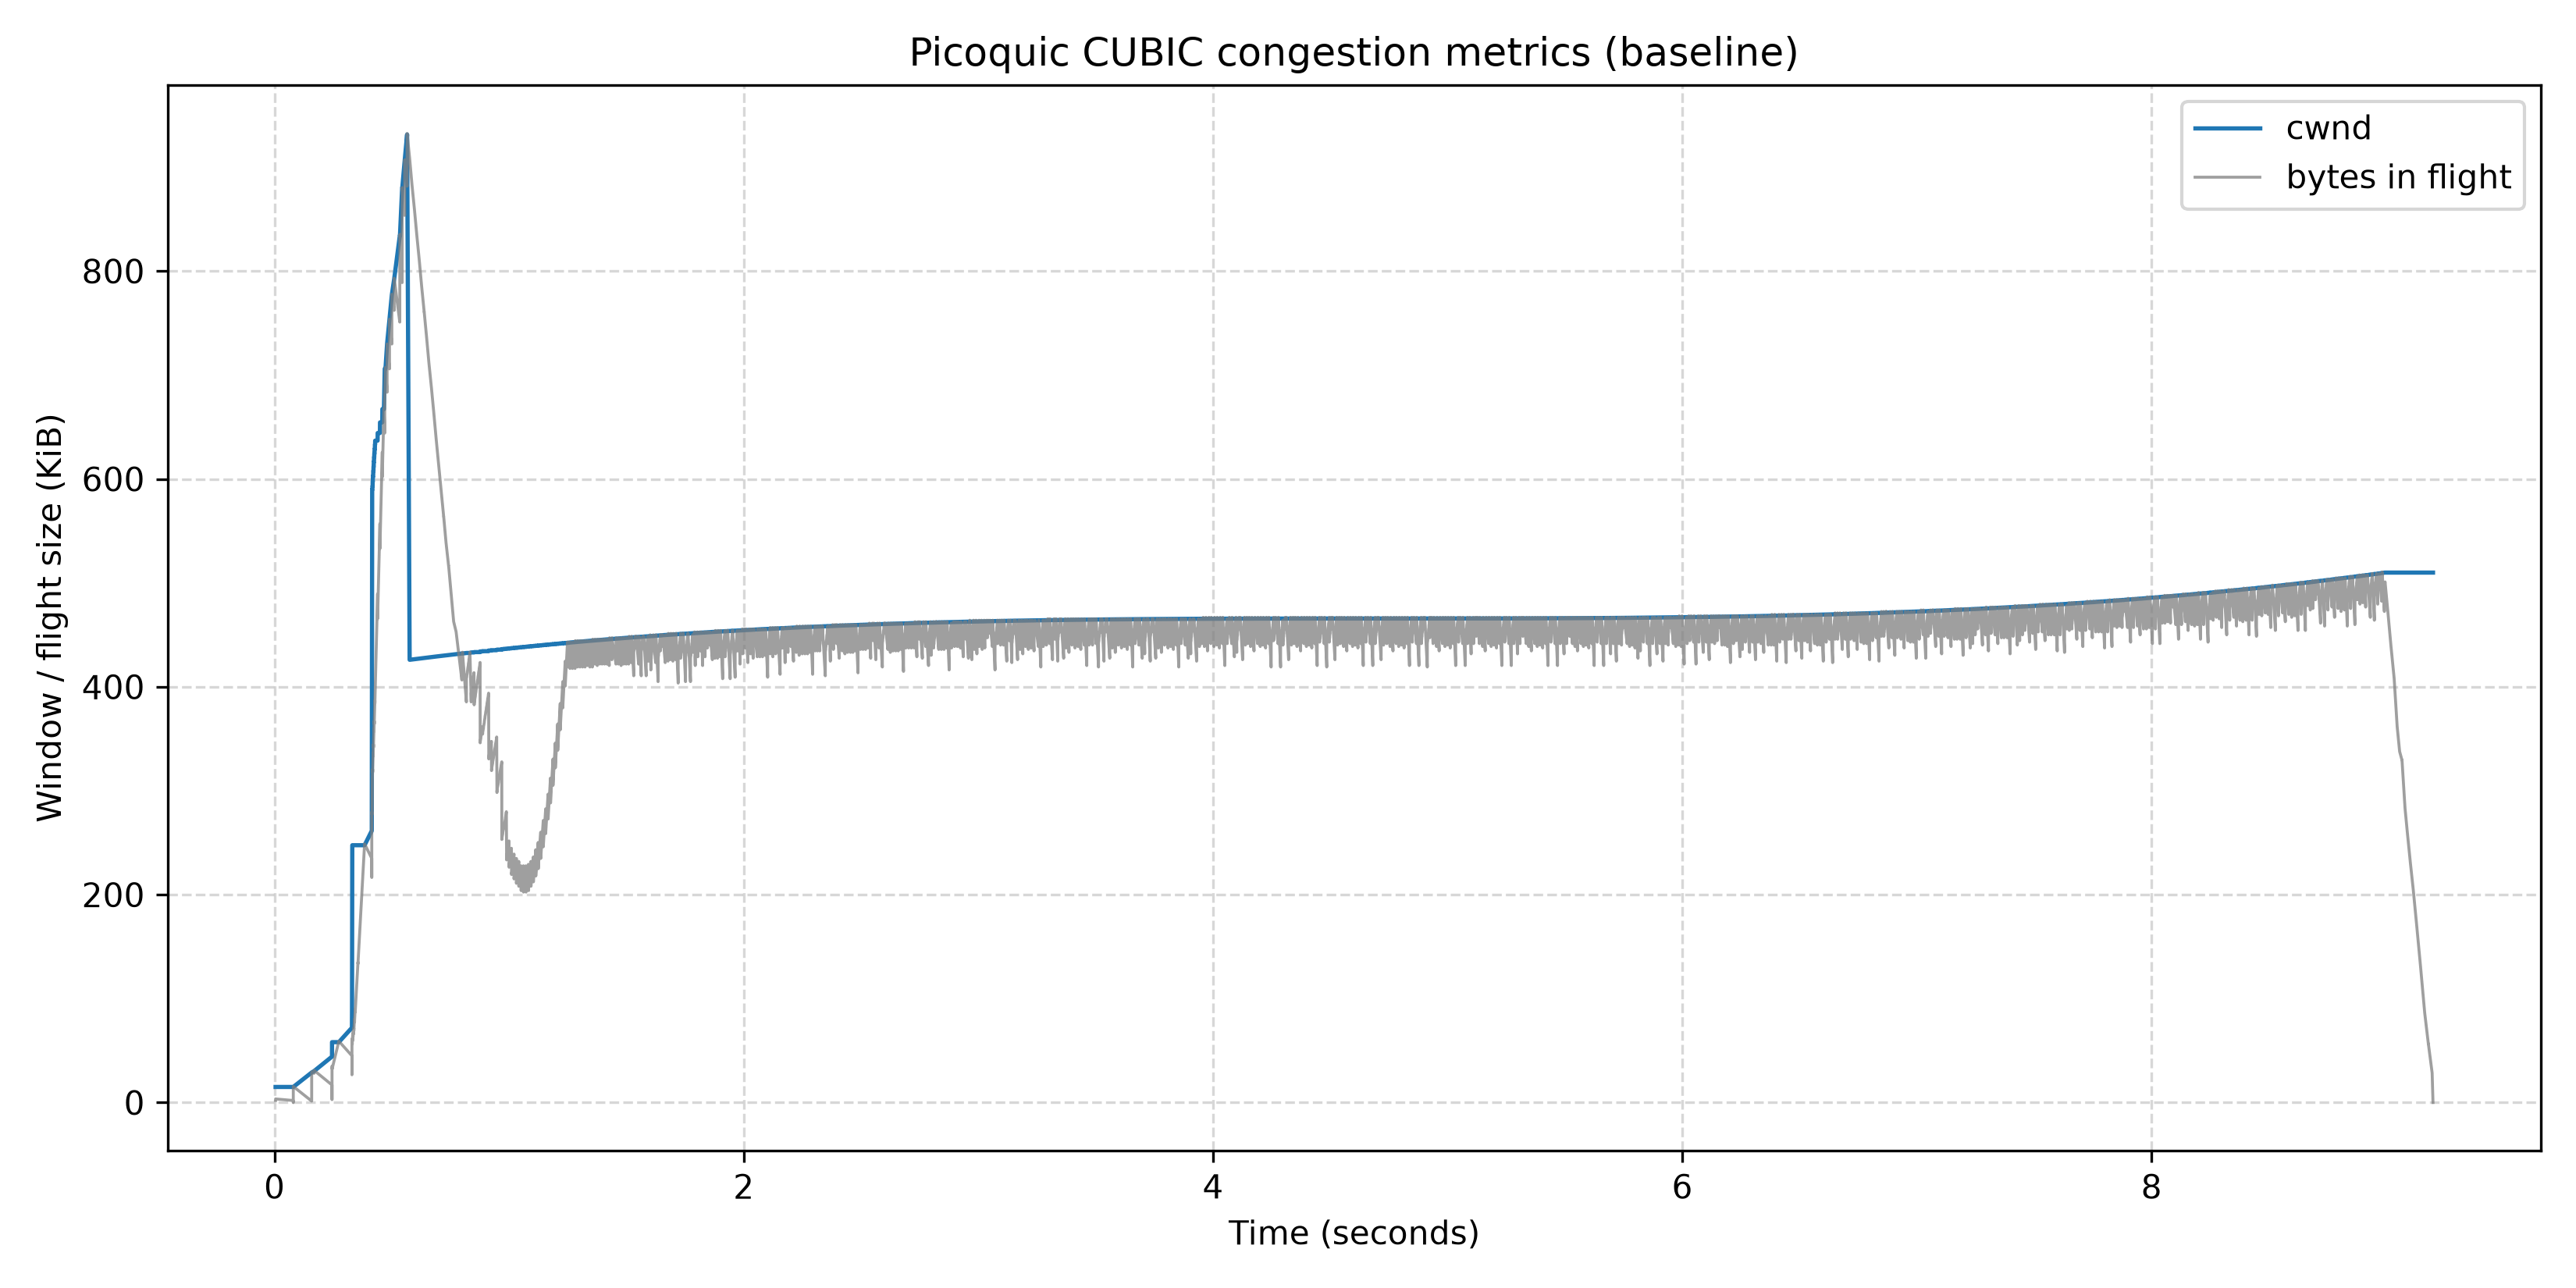
\includegraphics[width=0.92\textwidth]{plots/bulk-baseline-1.png}
\caption{Baseline: final cwnd 509.90 KiB; time-weighted mean 454.88 KiB; throughput 17.154 Mbit/s.}\end{figure}
\begin{figure}[H]\centering
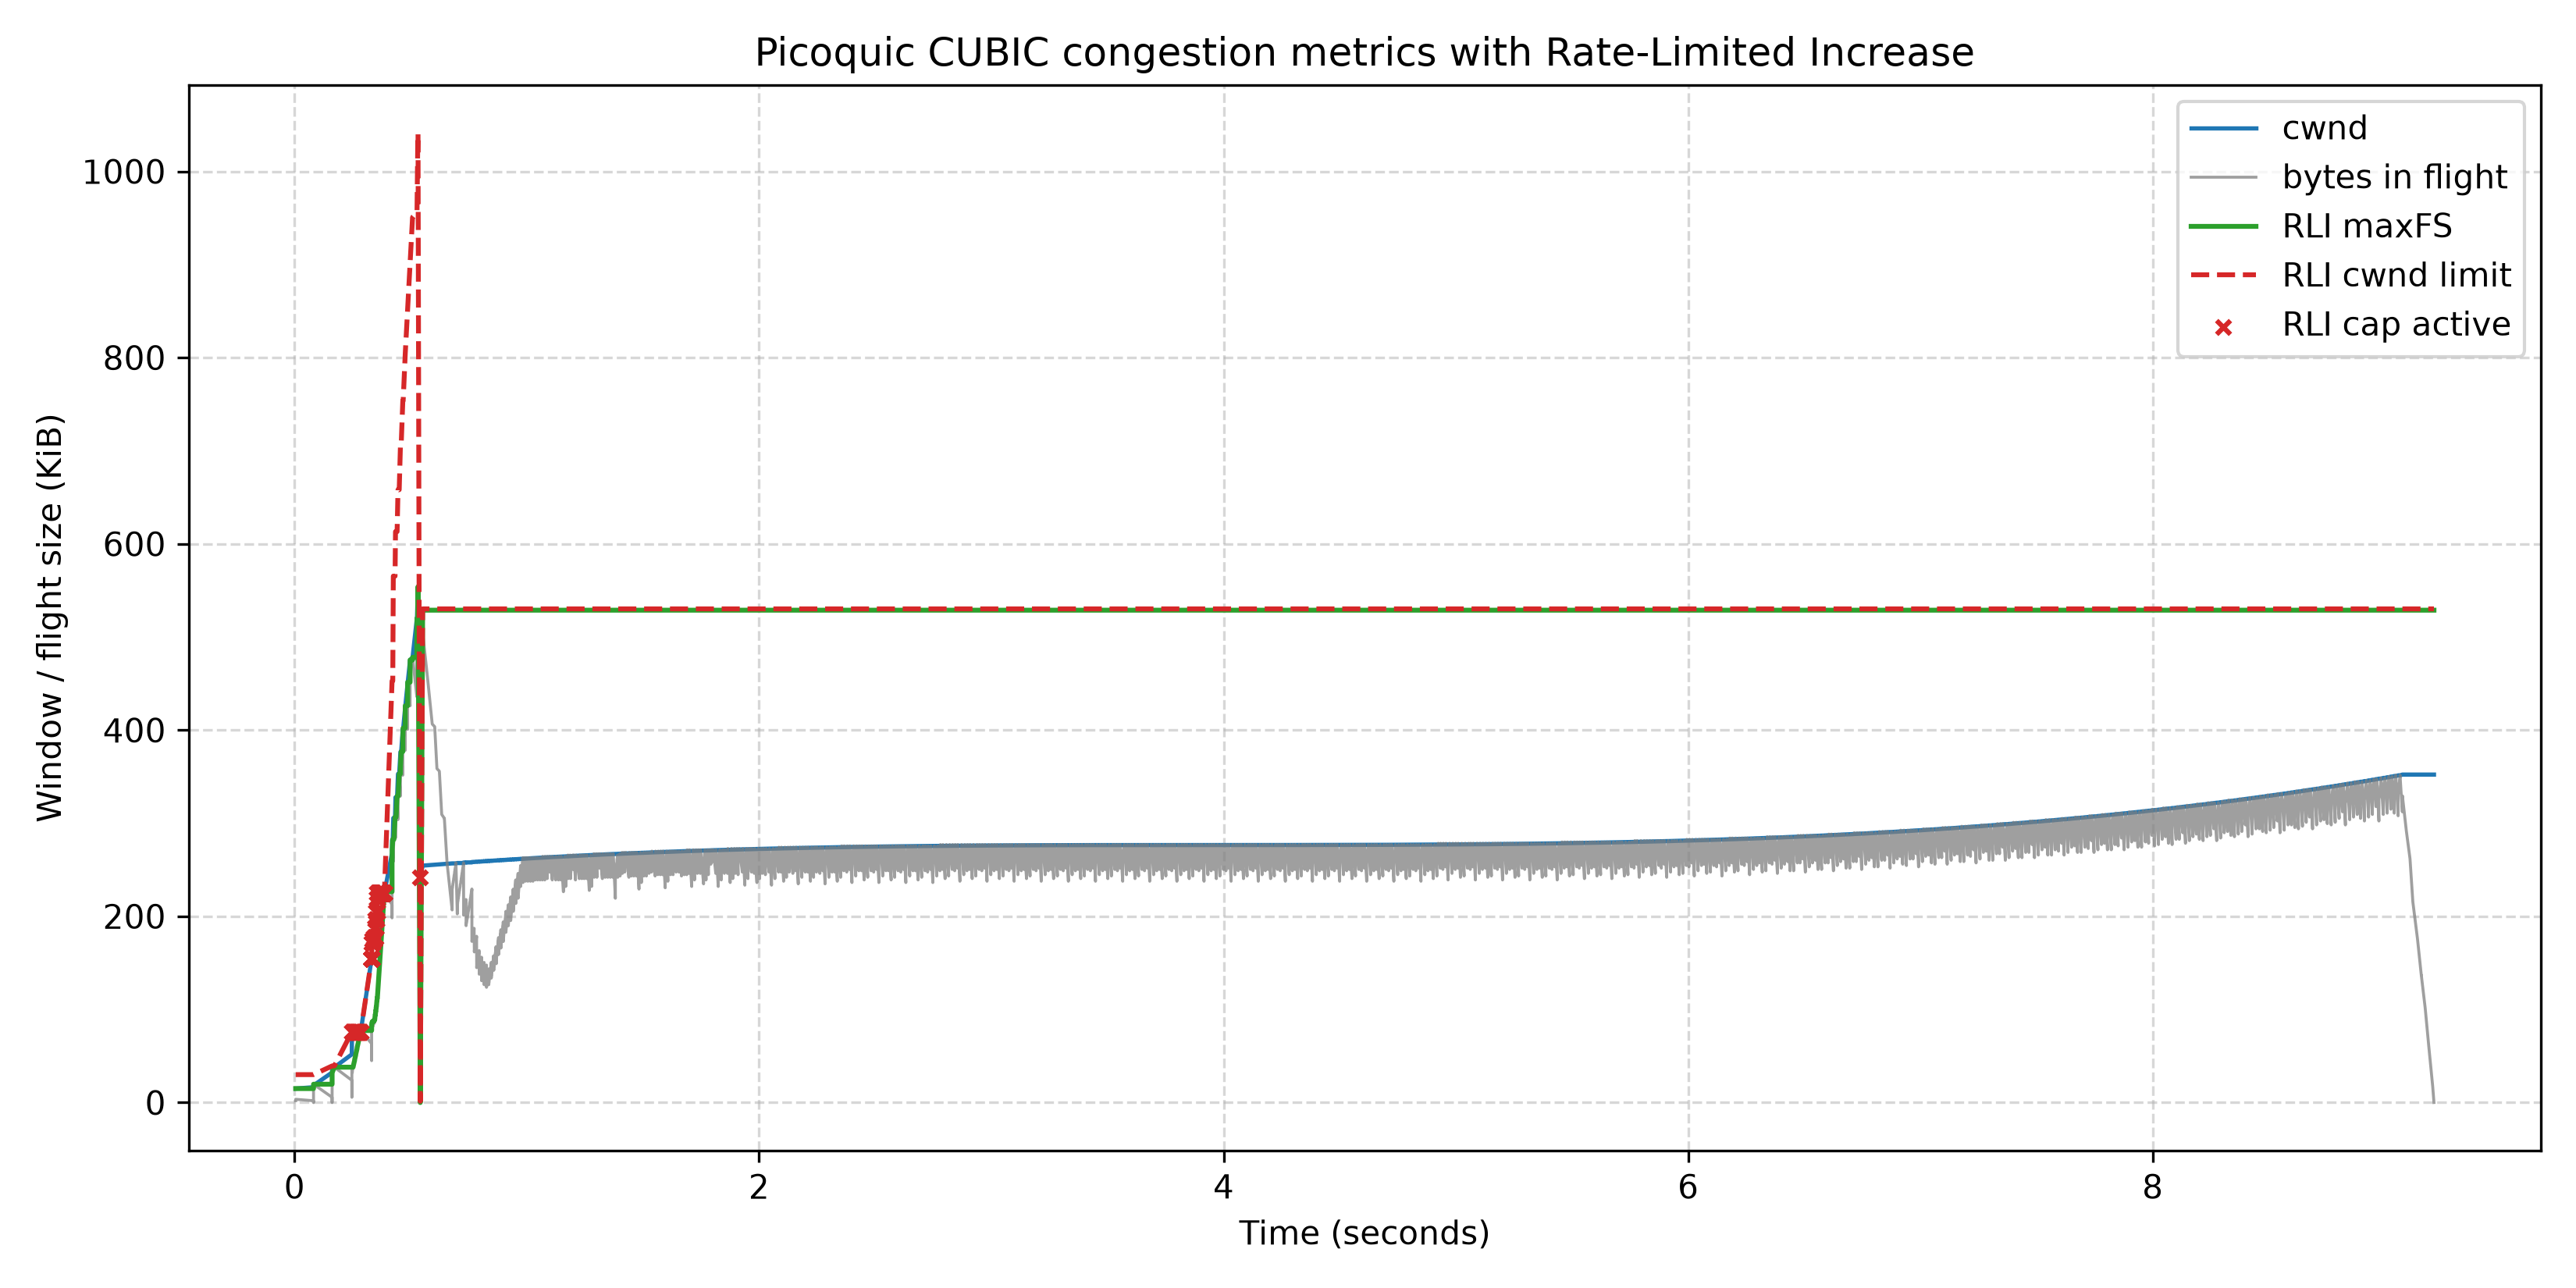
\includegraphics[width=0.92\textwidth]{plots/bulk-rli-1.png}
\caption{Rli: final cwnd 352.20 KiB; time-weighted mean 278.81 KiB; throughput 17.604 Mbit/s.}\end{figure}
These matched traces test a continuously backlogged sender. Normal CUBIC growth and congestion responses dominate; compare measured throughput rather than window height alone.
\clearpage\subsection{Bulk control, repetition 2}
\begin{figure}[H]\centering
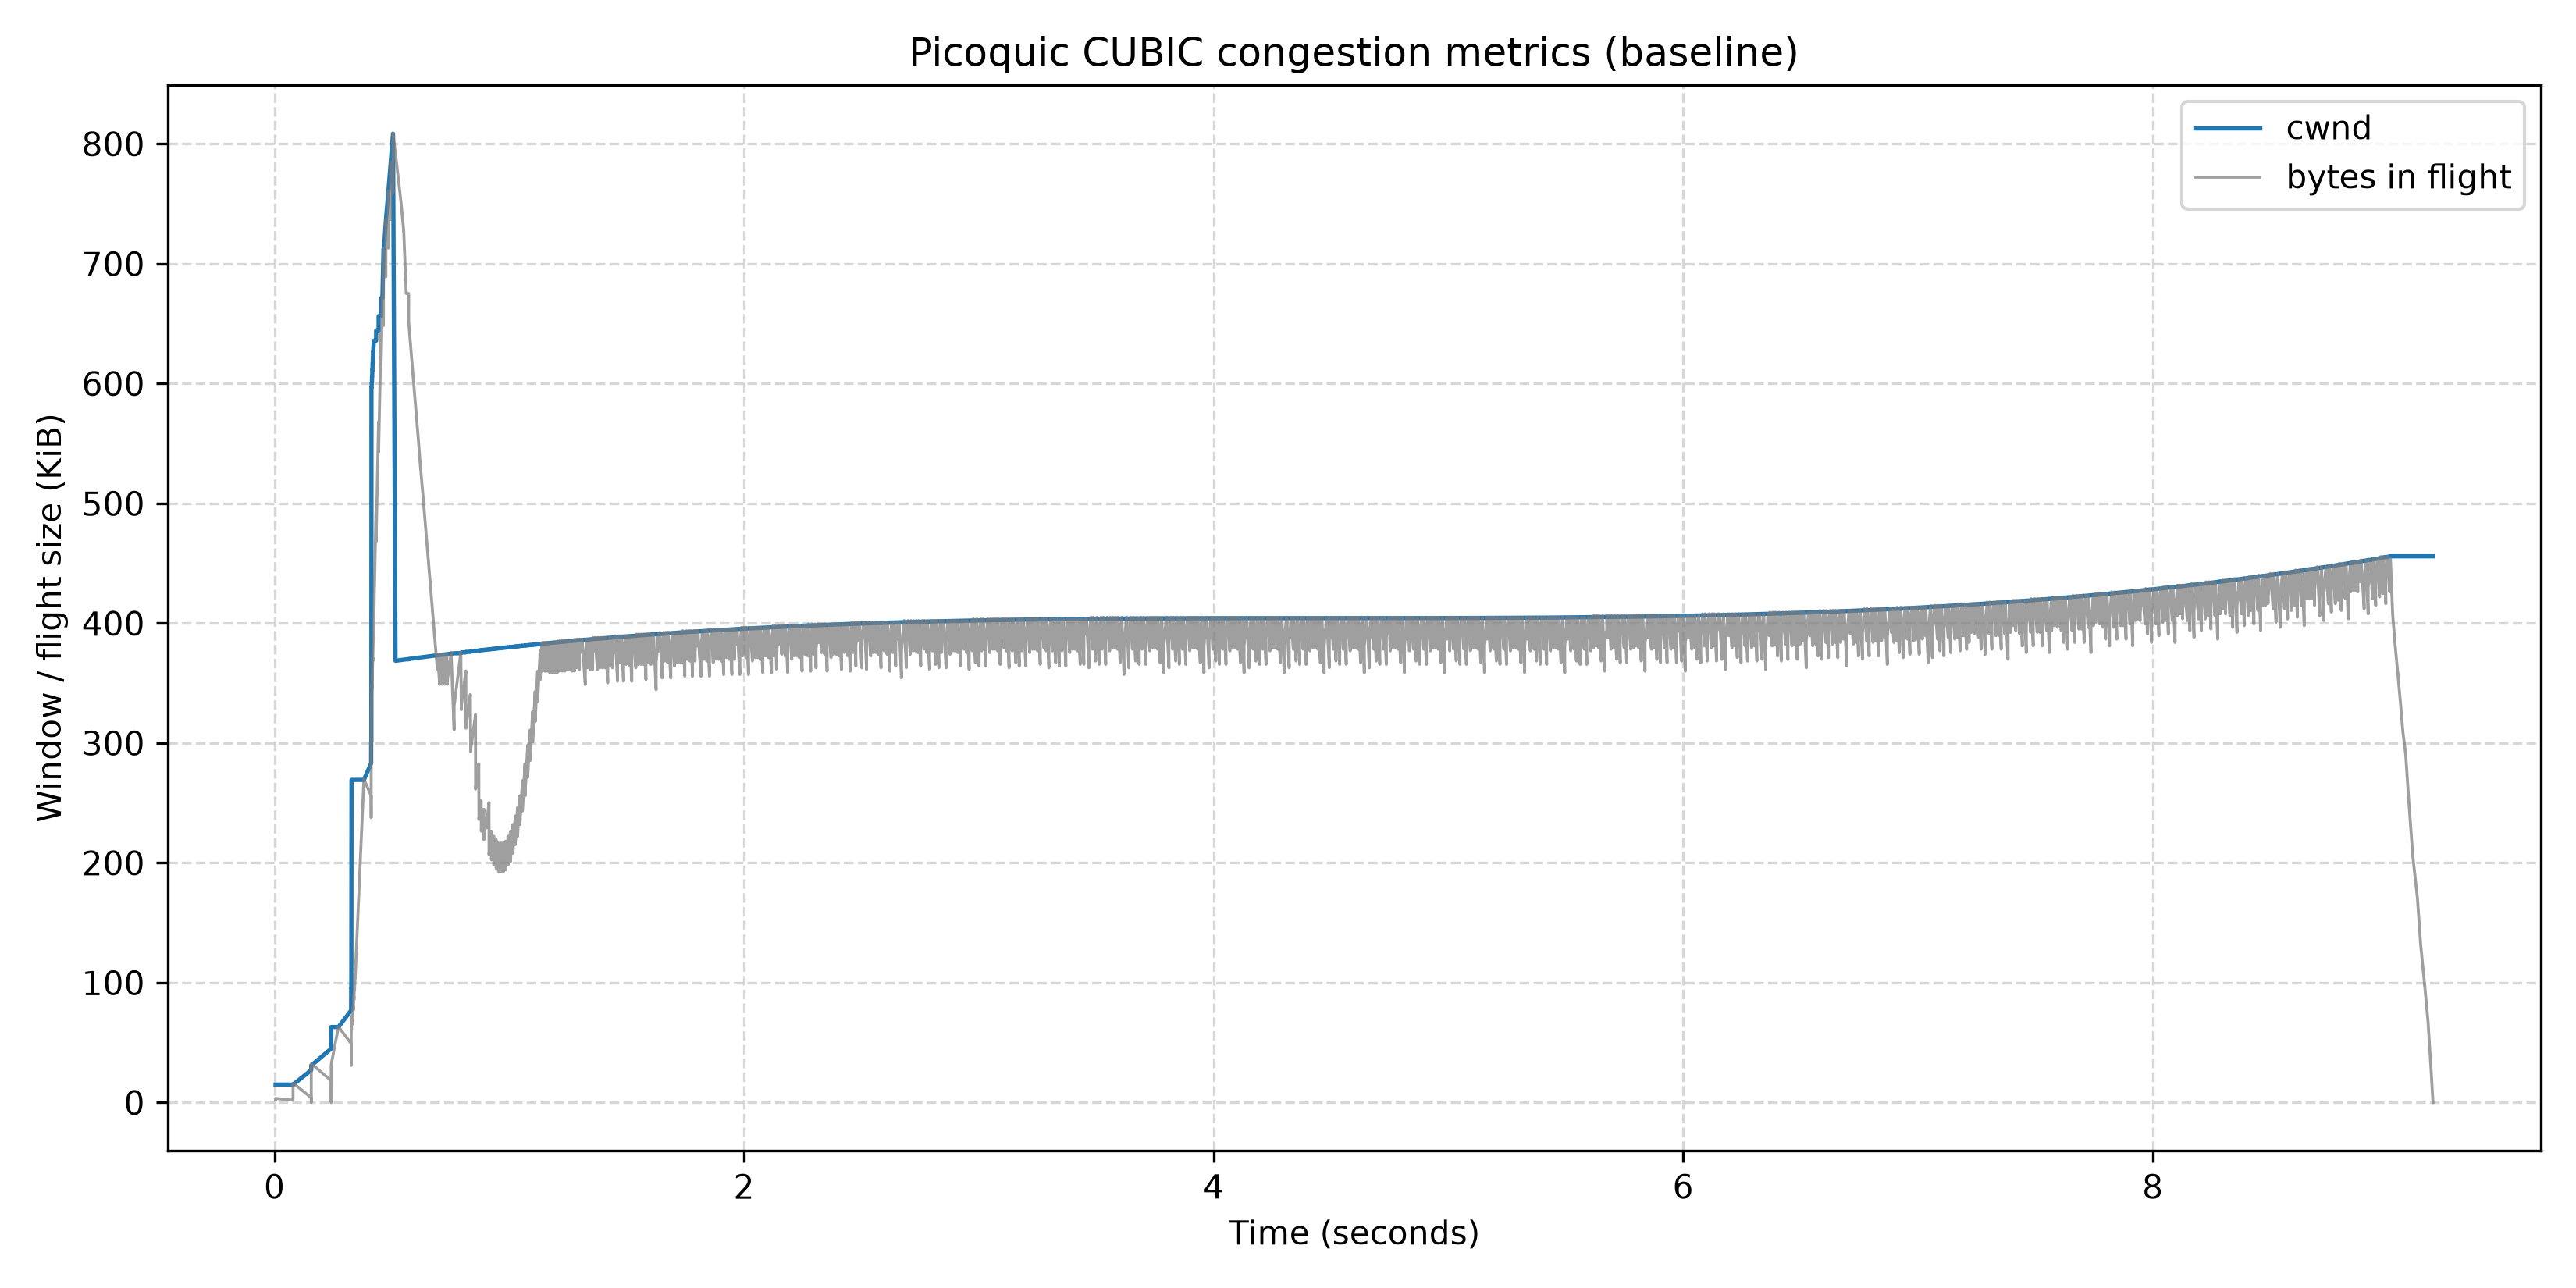
\includegraphics[width=0.92\textwidth]{plots/bulk-baseline-2.png}
\caption{Baseline: final cwnd 455.82 KiB; time-weighted mean 396.67 KiB; throughput 17.383 Mbit/s.}\end{figure}
\begin{figure}[H]\centering
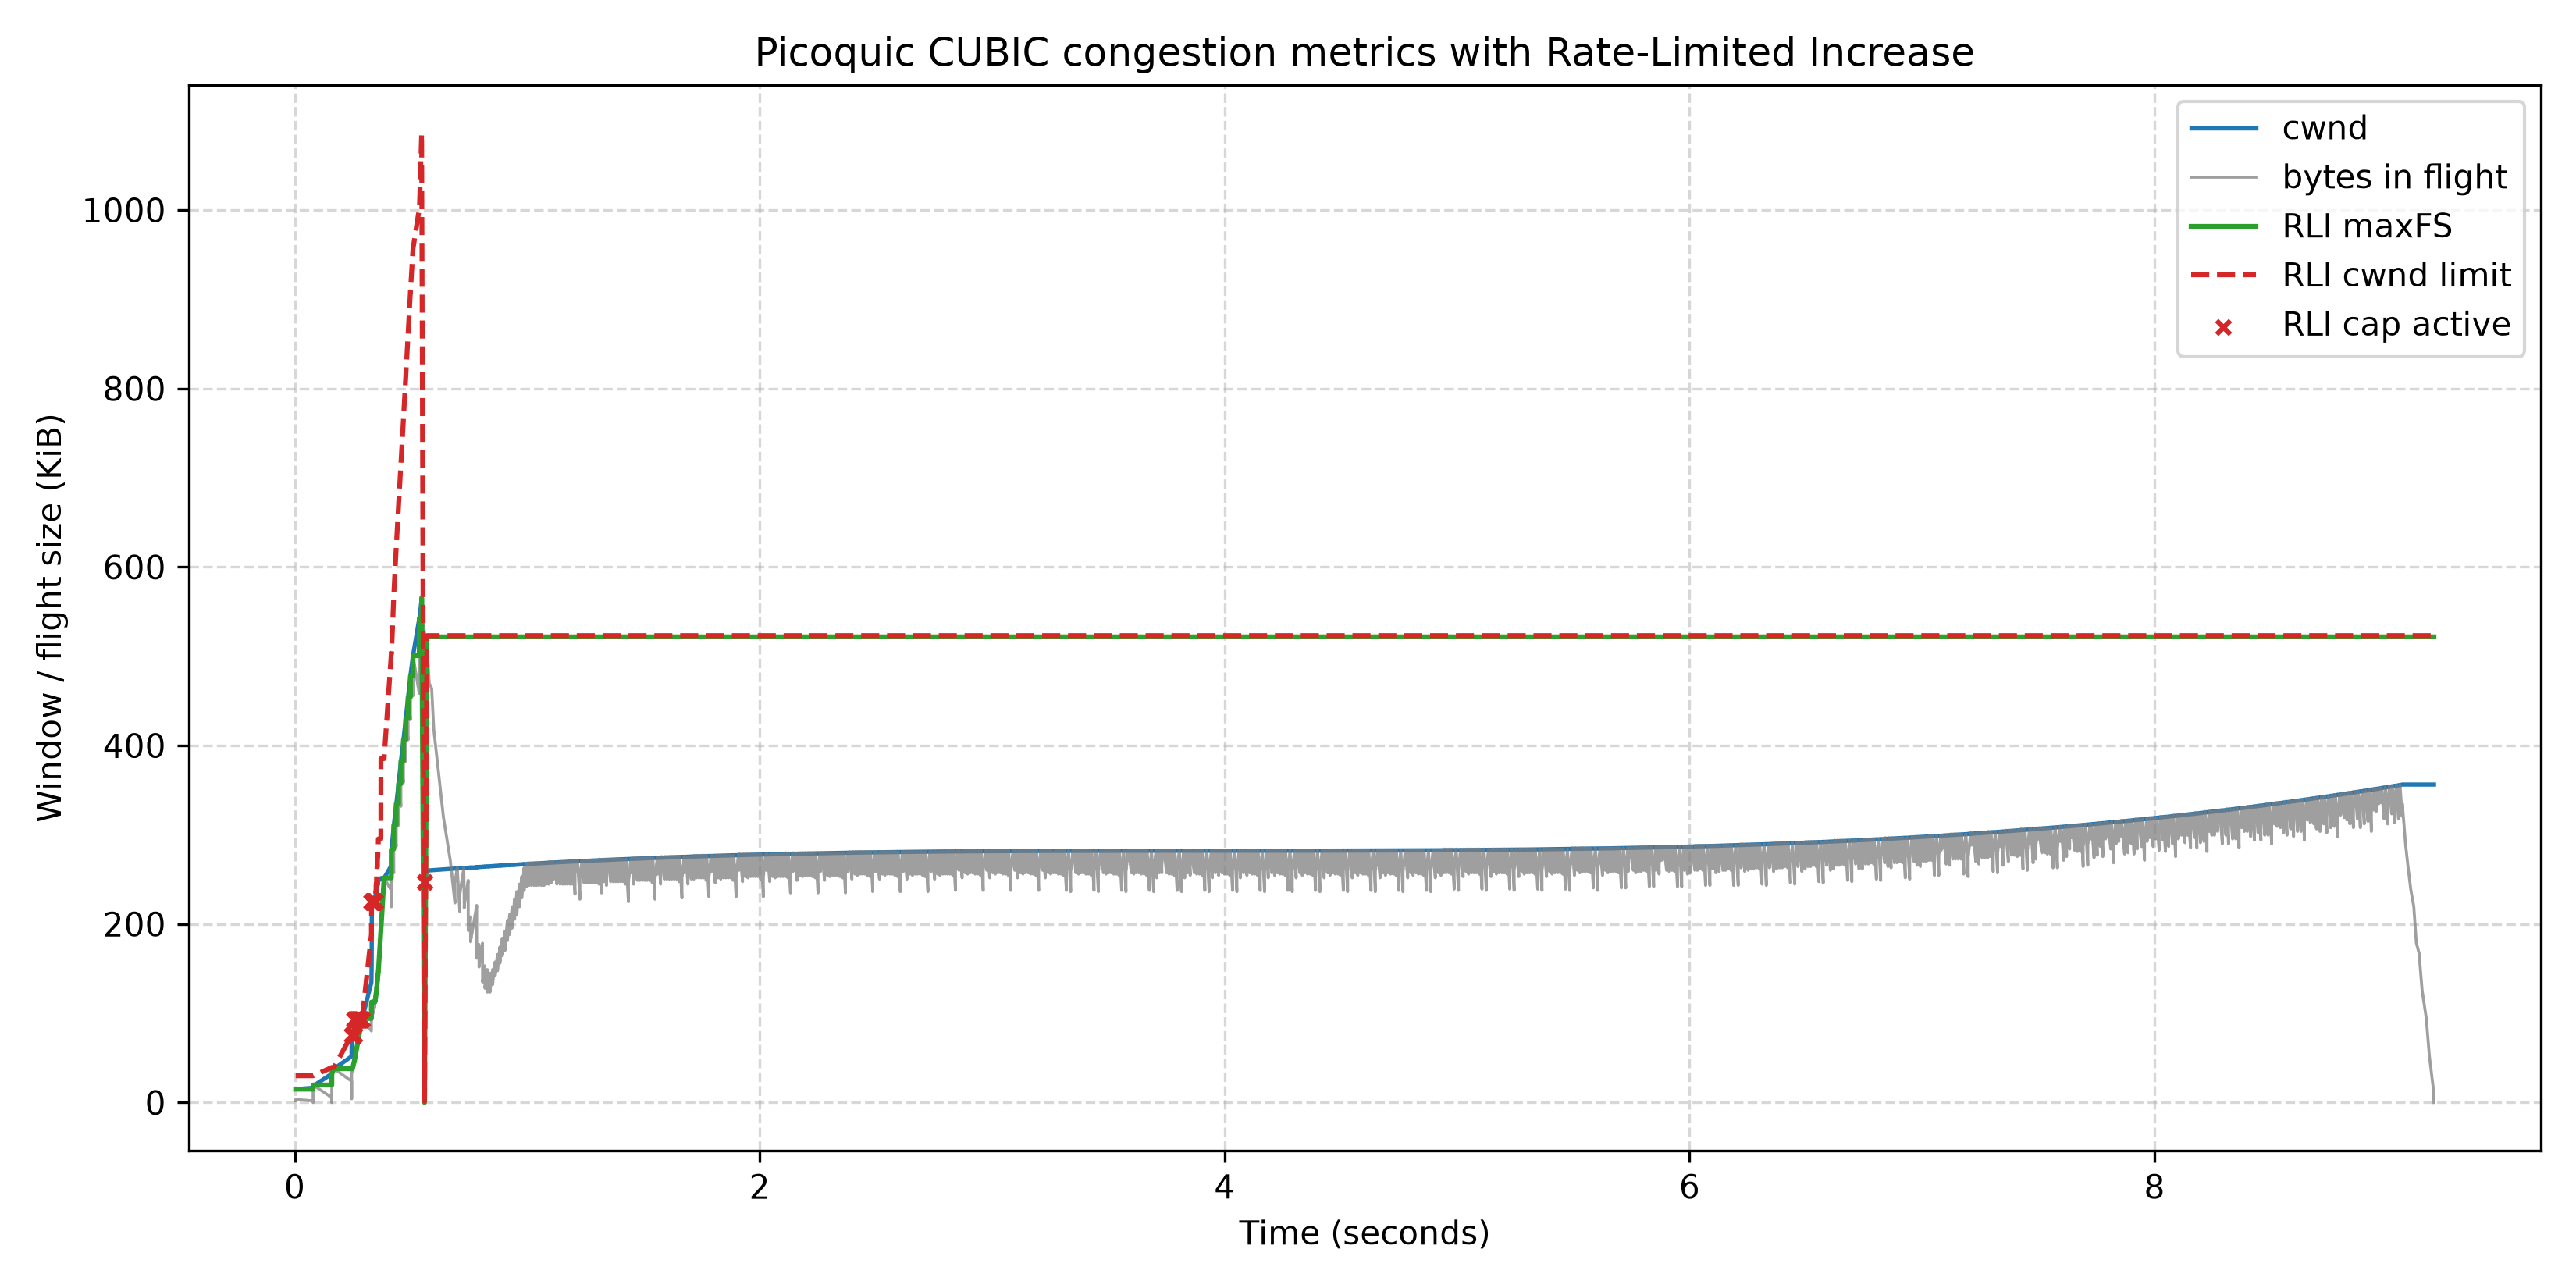
\includegraphics[width=0.92\textwidth]{plots/bulk-rli-2.png}
\caption{Rli: final cwnd 356.27 KiB; time-weighted mean 284.77 KiB; throughput 17.615 Mbit/s.}\end{figure}
These matched traces test a continuously backlogged sender. Normal CUBIC growth and congestion responses dominate; compare measured throughput rather than window height alone.
\clearpage\subsection{Bulk control, repetition 3}
\begin{figure}[H]\centering
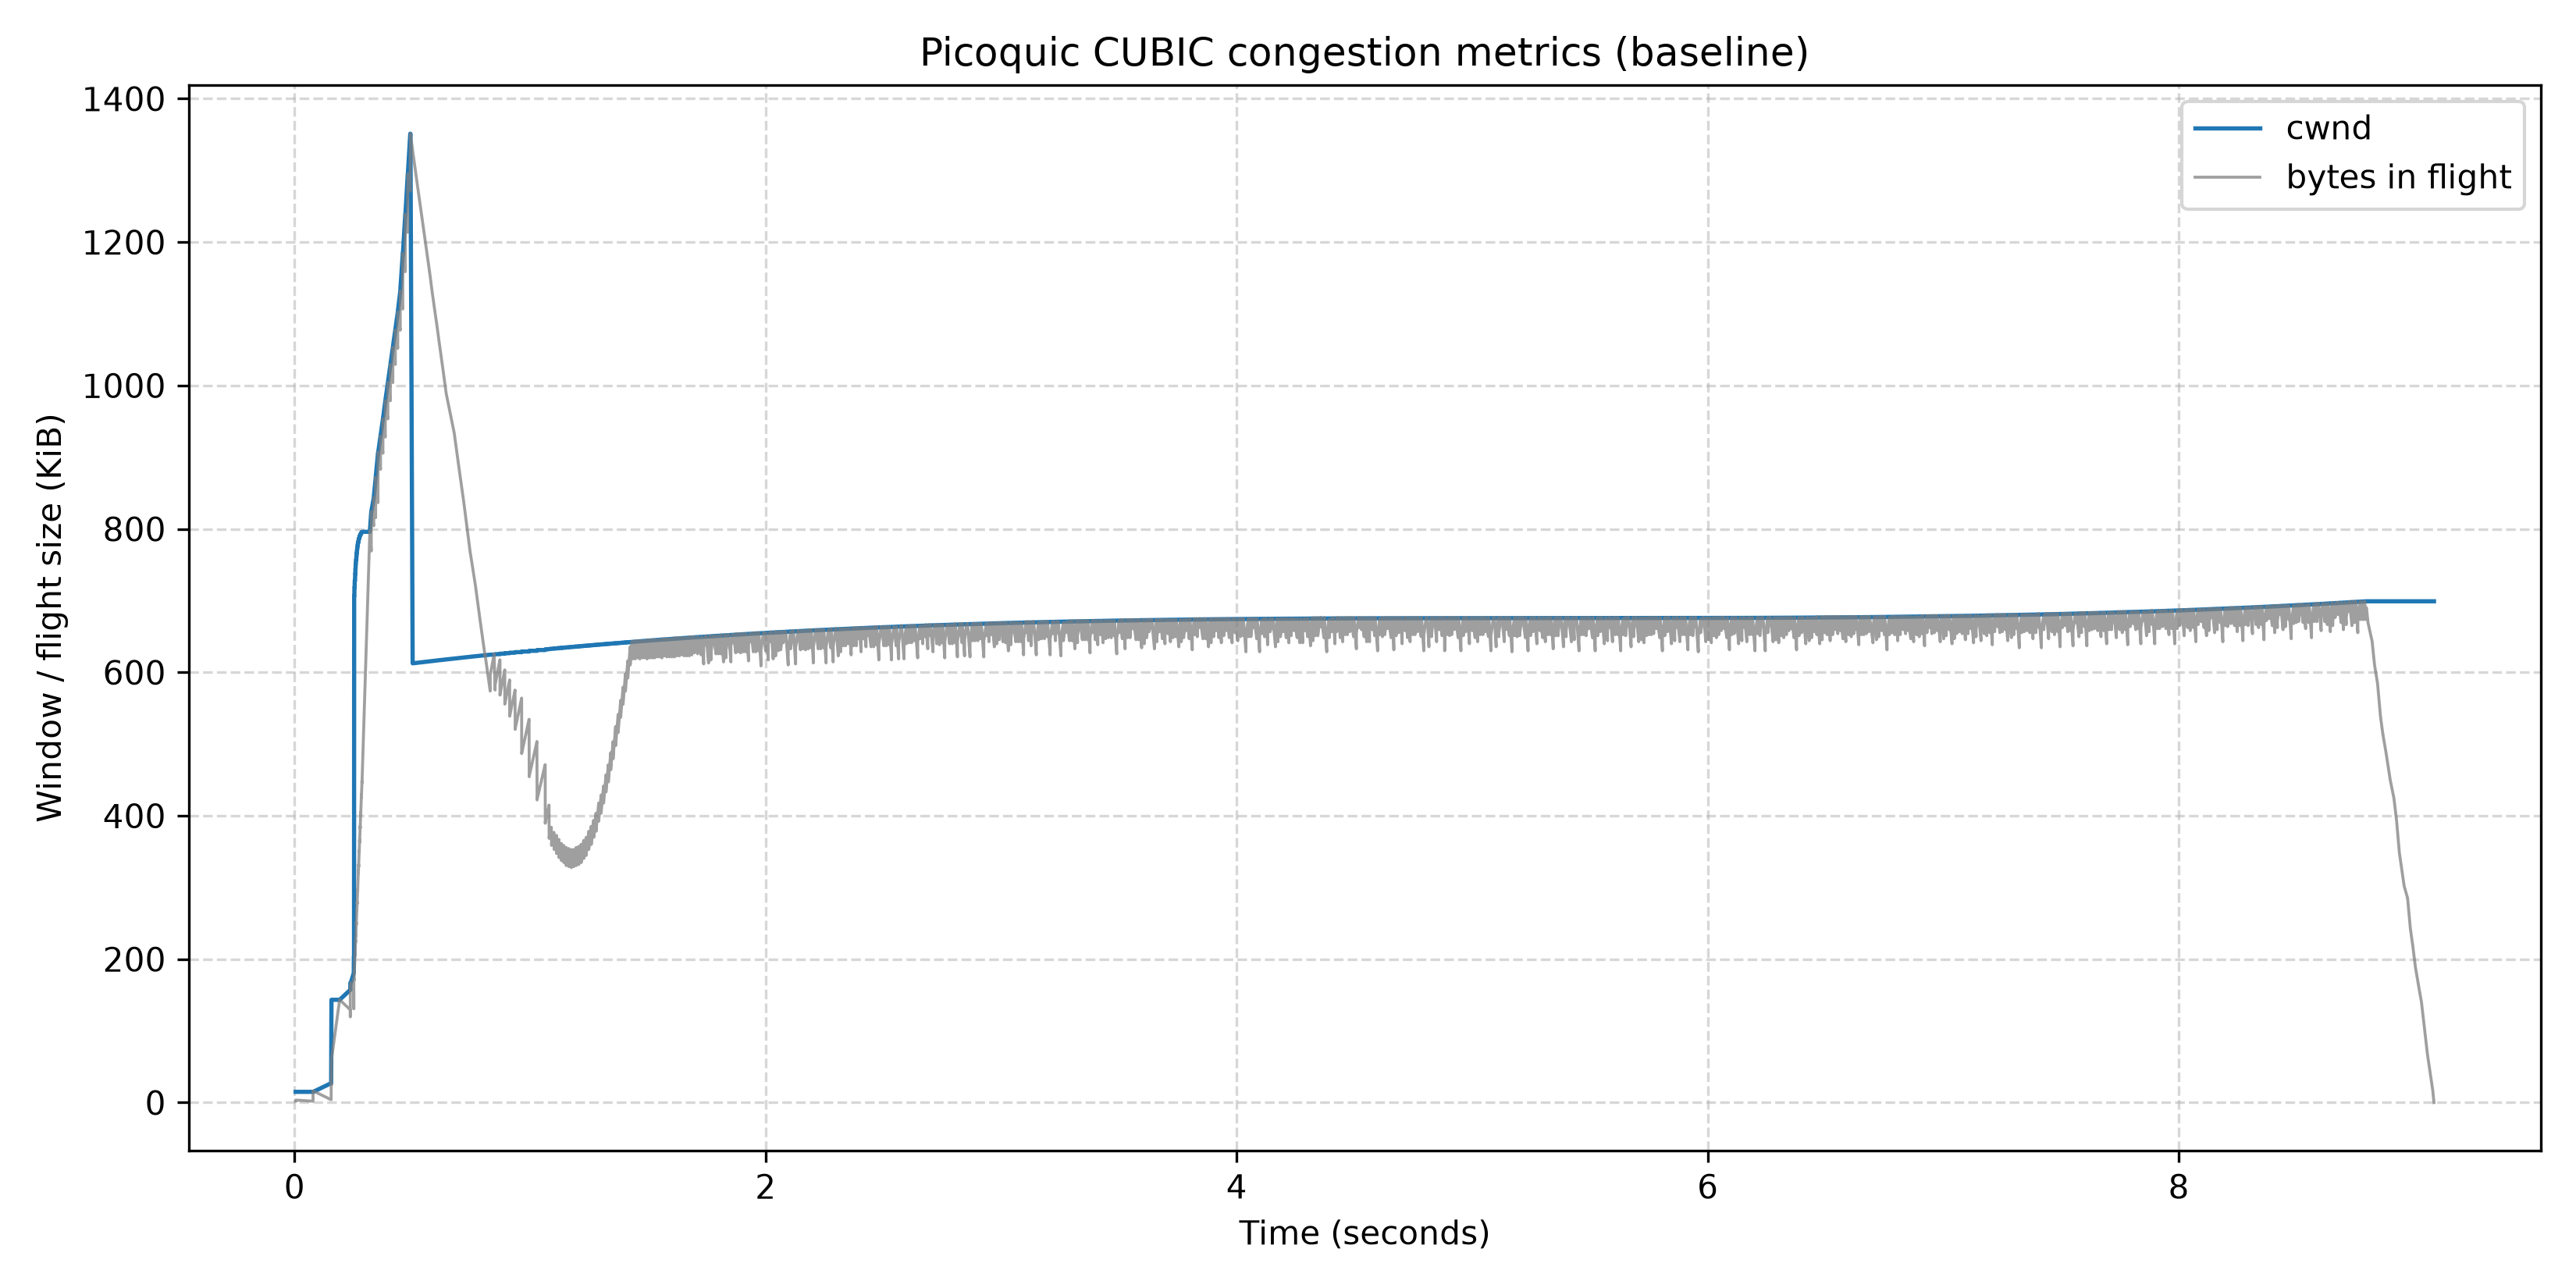
\includegraphics[width=0.92\textwidth]{plots/bulk-baseline-3.png}
\caption{Baseline: final cwnd 699.10 KiB; time-weighted mean 661.62 KiB; throughput 16.753 Mbit/s.}\end{figure}
\begin{figure}[H]\centering
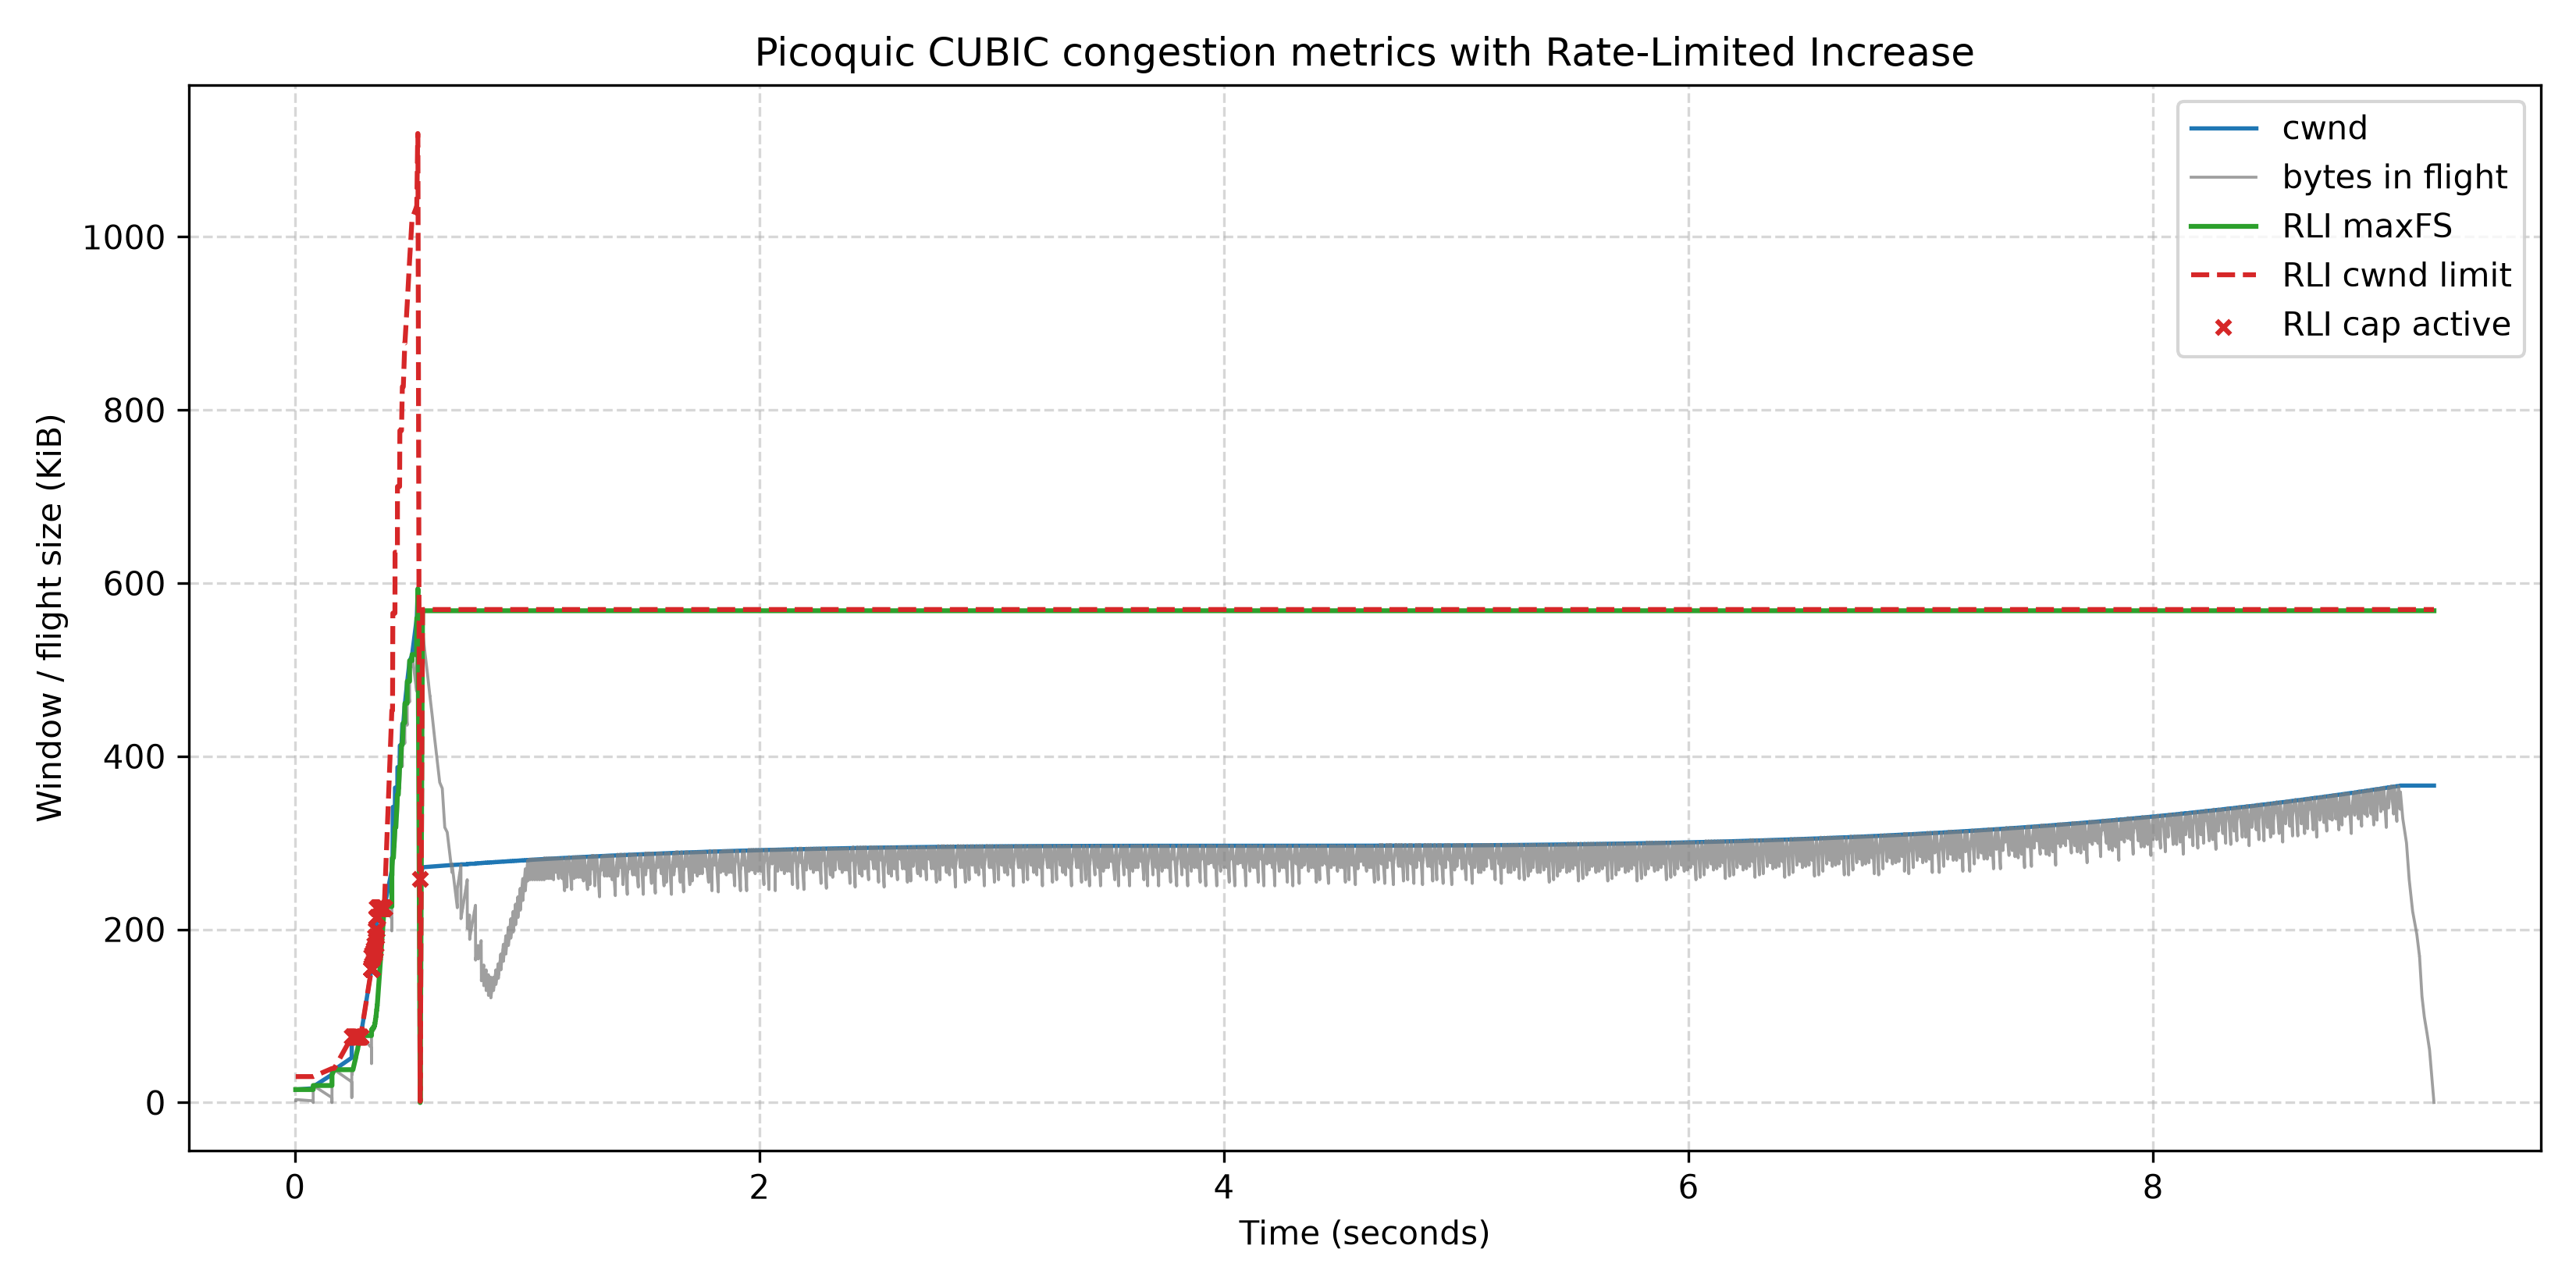
\includegraphics[width=0.92\textwidth]{plots/bulk-rli-3.png}
\caption{Rli: final cwnd 366.13 KiB; time-weighted mean 296.76 KiB; throughput 17.590 Mbit/s.}\end{figure}
These matched traces test a continuously backlogged sender. Normal CUBIC growth and congestion responses dominate; compare measured throughput rather than window height alone.
